% concatenated from tex/manuscript-journal.tex
\documentclass[twoside,11pt]{article}

\usepackage{blindtext}

% Any additional packages needed should be included after jmlr2e.
% Note that jmlr2e.sty includes epsfig, amssymb, natbib and graphicx,
% and defines many common macros, such as 'proof' and 'example'.
%
% It also sets the bibliographystyle to plainnat; for more information on
% natbib citation styles, see the natbib documentation, a copy of which
% is archived at http://www.jmlr.org/format/natbib.pdf

% Available options for package jmlr2e are:
%
%   - abbrvbib : use abbrvnat for the bibliography style
%   - nohyperref : do not load the hyperref package
%   - preprint : remove JMLR specific information from the template,
%         useful for example for posting to preprint servers.
%
% Example of using the package with custom options:
%
% \usepackage[abbrvbib, preprint]{jmlr2e}

\usepackage[preprint]{jmlr2e}


%%Packages
\usepackage{booktabs}
\usepackage{lipsum}
\usepackage{lgrmath} 
\usepackage{xcolor}   
%\usepackage{arevmath}
\usepackage{changepage}
\usepackage{amsfonts,amsmath,amsopn,amssymb}
\usepackage[scr=boondox,cal=esstix]{mathalpha}
\usepackage{graphicx}
\usepackage{epstopdf}
\usepackage{natbib}
\usepackage{algorithm, algpseudocode}
\usepackage{upgreek}
\usepackage{dsfont}
\usepackage{tikz}
\usepackage{tikz-cd}
\usepackage[T1]{fontenc}
\usepackage{tabularx,ragged2e}
\usetikzlibrary{arrows.meta, positioning, calc, shapes.geometric}
%\usepackage{cbfonts-fd}
\usepackage{subcaption}

%%Numbering
\numberwithin{equation}{section}
\numberwithin{theorem}{section}
\numberwithin{example}{section}


%%Macros
\newcommand{\degG}[1]{\deg\left(#1\right)}
\newcommand{\NN}[1]{\Gamma\left(#1\right)}
\DeclareSymbolFont{greekextras}{LGR}{cmr}{m}{it}
\def\multiset#1#2{\ensuremath{\left(\kern-.3em\left(\genfrac{}{}{0pt}{}{#1}{#2}\right)\kern-.3em\right)}}
\let\oldemptyset\emptyset
\let\emptyset\varnothing
\newcommand{\sho}{\textup{\text{\th}}}
\newcommand{\Sho}{\text{\TH}}
\newcommand{\Ngeod}[2]{\mathcal Q_{#1#2}}
\DeclareMathOperator*{\argmax}{arg\,max}
\DeclareMathOperator*{\argmin}{arg\,min}
\DeclareMathSymbol{\qoppa}{\mathord}{greekextras}{19} 
\DeclareMathSymbol{\Qoppa}{\mathord}{greekextras}{21}
\DeclareMathSymbol{\Koppa}{\mathord}{greekextras}{26} 
\newcommand{\Lip}{\operatorname{Lip}}
\newcommand{\nablaxy}[1]{\nabla_{xy}#1}
\newcommand{\nablayx}[1]{\nabla_{yx}#1}
\newcommand{\dataset}{{\cal D}}
\newcommand{\fracpartial}[2]{\frac{\partial #1}{\partial  #2}}
\makeatletter
\newcommand{\fullpagecenter}[1]{%
  \par\noindent
  \hspace*{-\@totalleftmargin}
  \makebox[\dimexpr\textwidth+\@totalleftmargin\relax][c]{#1}%
  \par
}
\makeatother

\definecolor{Accent}{HTML}{1F77B4}
\tikzset{
  v/.style      ={circle, fill=black, inner sep=1.0pt},             % generic vertex
  ring/.style   ={circle, draw=Accent, line width=0.7pt, fill=white, inner sep=1.0pt}, % counted vertex
  E/.style      ={line width=1.0pt, draw=Accent},                    % base edge e=(u,v)
  thin/.style   ={line width=0.45pt, draw=black!70},                 % ordinary adjacency
  cross/.style  ={line width=0.6pt, dashed, dash pattern=on 2pt off 1.2pt}, % cross edges (Xi)
  close/.style  ={line width=0.6pt, densely dotted},                 % k-closers (tildeBox)
  tag/.style    ={font=\scriptsize\itshape, fill=white, inner sep=1pt}
}

\newcommand{\BaseUV}{%
  \node[v,label=below:$u$] (u) at (0,0) {};
  \node[v,label=below:$v$] (v) at (2.9,0) {};
  \draw[E] (u)--(v);
}

% Unnumbered Lemma environment for local/auxiliary results
\makeatletter
\newenvironment{lemmast}[1][]%
  {\par\smallskip\noindent\textbf{Lemma%
     \@ifmtarg{#1}{}{ (\textbf{#1})}.\ }%
   \itshape}
  {\par\smallskip}
\makeatletter
%% Heading arguments are {volume}{year}{pages}{date submitted}{date published}{paper id}{author-full-names}
\usepackage{lastpage}
\usepackage{adjustbox}
\jmlrheading{XX}{2026}{1-\pageref{LastPage}}{XX/XX; Revised XX/XX}{XX/XX}{XX-XXXX}{Giorgio Micaletto, Tebe Nigrelli%
}

%% Short headings should be running head and authors last names
\ShortHeadings{Edgewise Envelopes Between Discrete Ricci Curvatures}{Micaletto and Nigrelli
}
\firstpageno{1}







\begin{document}

\title{Edgewise Envelopes Between Balanced Forman and Ollivier-Ricci Curvature}

\begingroup
\renewcommand\thefootnote{\fnsymbol{footnote}}
\setcounter{footnote}{0}

\author{\name Giorgio Micaletto
        \email gmicaletto@uchicago.edu\\
        \addr Department of Statistics\\
        University of Chicago\\
        Chicago, IL 60637-1514, USA
        \AND 
        \name Tebe Nigrelli
        \email tebe.nigrelli@studbocconi.it\\
        \addr Department of Computing Sciences\\ 
        Bocconi University\\
        Via Roberto Sarfatti 25, 20136 Milan, Italy
}
\begingroup
\makeatletter
\renewcommand\@makefntext[1]{%
\noindent\makebox[1.8em][r]{\!\@makefnmark:}\,#1%
}
\makeatother
\endgroup
\endgroup


\editor{
%None 
}

\maketitle


\begin{abstract}
Evaluating Ollivier-Ricci (OR) curvature on large-scale graphs is computationally prohibitive due to the necessity of solving an optimal transport problem for every edge. We bypass this bottleneck by deriving explicit, two-sided, piecewise-affine transfer moduli between the transport-based OR curvature and the combinatorial Balanced Forman (BF) curvature. We establish deterministic bounds for $\mathfrak{c}_{\rm OR}(i,j)$ parameterized by 2-hop local graph combinatorics, 
reducing the edgewise evaluation complexity from an optimal transport linear program to a worst-case $\mathcal{O}(\max_{v \in V} \deg(v)^{2.5})$ time, entirely eliminating the reliance on global solvers.
Empirical scalability benchmarks confirm these theoretical guarantees, demonstrating that the proposed transfer moduli yield significant asymptotic and constant-factor speedups over the steep polynomial scaling of exact OR evaluation. 
Furthermore, the tightness of these bounds is validated via distributional analyses on canonical random graphs and empirical networks, with the derived analytical bands enclosing the empirical distributions independent of degree heterogeneity, geometry, or clustering, providing a scalable, computationally efficient framework for rigorous statistical network analysis.
\end{abstract}
\begin{keywords}
Ollivier--Ricci curvature; Balanced Forman curvature; scalable network analysis; computational graph theory; optimal transport on graphs; empirical curvature distributions.
\end{keywords}

%\begin{AMS}
%Primary: 49Q22; Secondary: 05C12, 05C81, 05C21, 60J10, 68R10.
%\end{AMS}

\section{Introduction}
\label{sec:introduction}
Discrete analogues of Ricci curvature on graphs have become fundamental tools in both network science and geometric deep learning. Two main families account for the majority of papers in this area: (i) transport-based coarse Ricci curvatures \citep{ollivier_ricci_2009, lin_curvature_2011}, (ii) combinatorial curvatures \citep{forman_method_2003,sreejith_forman_2016,weber_forman_2016,samal_comparative_2018}.

In geometric graph analysis and graph neural networks (GNNs), OR curvature is increasingly utilized to identify structural bottlenecks, where modifying the graph topology based on curvature signs can simultaneously resolve over-squashing and over-smoothing phenomena \citep[e.g.][]{nguyen_over_2023,liu_curvdrop_2023}. However, evaluating exact OR curvature requires solving a Wasserstein optimal transport problem for every edge., which severely limits the scalability of principled, geometry-aware algorithms on large datasets. 

The literature includes several empirical studies comparing these discrete curvature notions across graph models and real networks, often reporting substantial, but not universal, agreement while also highlighting regimes where they differ \citep{sreejith_systematic_2017, samal_comparative_2018, saucan_discrete_2018}. 

Recent work has attempted to reconcile these two perspectives: \citet{topping_squashing_2022} introduced BF curvature, a combinatorial edge-based notion that provides a sharp one-sided lower bound for \cite{lin_curvature_2011} curvature on graphs, while other studies have proposed extensions of Forman curvature aimed at bringing it into closer alignment with OR in applications \citep{tee_enhanced_2021, samal_comparative_2018}.

\paragraph{Positioning of This Work.}
To the best of the authors' knowledge, despite many empirical comparisons and one-sided bounds, there is no \emph{analytic, two-sided} relation between transport-based and combinatorial curvatures at the \emph{edge level} on general graphs.
While approximate solvers like Sinkhorn-Knopp \citep[e.g.,][]{knight_sinkhorn_2008} offer 
$\mathcal{O}\left((\max_{v\in V}\deg(v)/ \epsilon)^2\right)$ scaling for the transport step, they require constructing a dense local distance matrix, a $\mathcal{O}(\max_{v\in V}\deg(v)^3)$ bottleneck, and introduce entropy regularization that destroys the deterministic guarantees required for exact bounding.
Our contribution is (i) to develop a \emph{lazy transport envelope} that upper-bounds the edgewise Wasserstein-1 yielding an envelope for OR curvature as a function of degrees, laziness, triangle count, and a 4-cycle coverage (Proposition \ref{prop:lazy-envelope-sharpened}) and (ii) computing a \emph{necessary triangle threshold} that turns OR bounds into BF bounds.

\paragraph{What We Mean by ``Transfer Moduli''.}
We define \emph{edgewise transfer moduli} as pairs of nondecreasing functions, \(\varphi^{(i,j)}\) and \(\psi^{(i,j)}\), that convert a bound on one curvature into a bound on the other. 
For $\mathfrak c_{\rm BF} \mapsto \mathfrak c_{\rm OR}$, and symmetrically for $\mathfrak c_{\rm OR} \mapsto \mathfrak c_{\rm BF}$, we require:
\[
\begin{aligned}
 \mathfrak c_{\rm BF}(i,j)\ge \zeta \ \implies\mathfrak c_{\rm OR}(i,j)\ge \varphi^{(i,j)}_{\rm BF \to OR}(\zeta),\\
 \mathfrak c_{\rm BF}(i,j)\le \vartheta \ \implies \mathfrak c_{\rm OR}(i,j)\le \psi^{(i,j)}_{\rm BF \to OR}(\vartheta).
\end{aligned}
\]
Crucially, because these functions depend solely on 2-hop neighborhoods, they are explicit and computable in worst-case $\mathcal{O}(\max_{v\in V}\deg(v)^{2.5})$ time per edge, completely bypassing the optimal transport linear program, and as GNNs primarily rely on identifying extreme curvature values to rewire graphs, these envelopes allow practitioners to flag geometric bottlenecks efficiently, making scalable OR-based network analysis computationally tractable.

\paragraph{Distributional Predictions and Experimental Scope.}
Our experimental evaluation is twofold: validating the computational scaling of our local combinatorial approach against exact solvers, and understanding \emph{how} curvatures are distributed across different topologies. For the latter, we examine full empirical \emph{histograms} of OR and BF curvature against our transfer bounds, which act as analytical envelopes for the observed distributions, complementing prior comparative work that emphasized edgewise scatter plots and rank correlations \citep{sreejith_systematic_2017, samal_comparative_2018}. We benchmark across three families of testbeds to isolate distinct drivers of curvature: \emph{random graph models} that control degree heterogeneity, clustering, and geometry \citep{erdos_random_1959,watts_collective_1998,barabasi_emergence_1999,penrose_random_2003,steger_generating_1999,holland_stochastic_1983,krioukov_hyperbolic_2010}; \emph{canonical combinatorial families} that provide clean baselines and extremes (\emph{Cycles}, \emph{Rectangular grids}, \emph{$d$-ary trees}, and \emph{Complete graphs}); \emph{real networks} that supply heterogeneous, noisy ground truth \citep{zachary_karate_1977,gleiser_community_2003,watts_collective_1998,milo_motifs_2002,gehrke_arxiv_2003}.

This allows us to evaluate our transfer bounds against degree control, clustering, geometry, community structure, and real-world heterogeneity. As demonstrated in Section~\ref{sec:analysis}, our approach yields orders-of-magnitude execution speedups while ensuring the analytical bands enclose the empirical distributions regardless of the underlying structural complexities.


\section{Preliminaries}
\label{sec:prelims}
\begin{remark}
Proofs of all stated results are provided in Appendix~\ref{appendix:proofs}.
\end{remark}
In the following, we fix the notation, collect the basic objects used for transport, the curvature notions of interest, and the combinatorial summaries that parameterize our explicit couplings and bounds used in the next sections. We work with a simple (undirected, loopless, no multi-edges), finite, connected graph \(G=(V,E)\), where $n:=|V|$ and degrees are defined as
\(
\varrho_u:=\deg_G(u)=|\mathcal N(u)|,
\)
where $\mathcal N(u)$ denotes the set of vertices adjacent to $u$,
\(
\mathcal N(u):=\{v\in V:(u,v)\in E\}.
\)



\begin{definition}[Lazy Random-Walk Measure]
\label{def:lazy-rw}
For \(u \in V\), define the \emph{one-step (lazy) random-walk measure} on \(V\) by
\(
m_u :=\; \alpha_u\,\delta_u \;+\; (1-\alpha_u)\,\nu_u,
\)
where \(
\alpha_u = (\varrho_u + 1)^{-1},
\)
\(\delta_u\) denotes the \emph{Dirac mass} at \(u\) (\(
  \delta_u(k) := \mathds{1}_{\{k=u\}} (k)
  \)), and  \(\nu_u\) is the \emph{random-walk adjacency measure} at \(u\), defined as
  \(
  \nu_u(k) := {\varrho_u}^{-1}\mathds{1}_{\{k\in\mathcal N(u)\}}
  \)
\end{definition}


\begin{remark}[Saturating the Diagonal]
\label{rem:saturate-diagonal}
Let $(V,\mathrm{dist}_G)$ be a finite metric space and let $\mathcal P(V)$ denote the set of probability measures on $V$; given $\mu,\nu\in\mathcal P(V)$, let $\gamma:V\to[0,1]$ be the common mass
$\gamma(x):=\min\{\mu(x),\nu(x)\}$. By \emph{saturating the diagonal} we mean the operation
of first assigning
\(
\pi(x,x) \leftarrow \gamma(x)
\)
for all $x\in V$,
and then coupling only the residual measures
$\mu^{\perp}:=\mu-\gamma$ and $\nu^{\perp}:=\nu-\gamma$, which have disjoint supports.
This doesn't change nor increase the optimal cost,
\(
W_1(\mu,\nu)=W_1(\mu^{\perp},\nu^{\perp}),
\)
as mass placed on the diagonal incurs zero transportation cost.
\end{remark}

Table~\ref{tab:definitions} formally establishes the primary neighborhood sets, and combinatorial parameters associated with an arbitrary edge \(e=(i,j) \in E\), with the underlying geometric motifs governing these parameters illustrated in Figure~\ref{fig:local-summaries}.


\begin{table}
\caption{Definitions, neighbor measures, and lazy transport parameters evaluated for a fixed edge $e=(i,j) \in E$.}
\label{tab:definitions}
\centering
\small
\renewcommand{\arraystretch}{1.3}
\begin{tabular}{@{}p{0.3\textwidth}p{0.7\textwidth}@{}}
\toprule
\textbf{Concept / Symbol} & \textbf{Definition / Formula} \\
\midrule
\textbf{Neighborhood Sets} & Common: $\mathcal C := \mathcal N(i)\cap\mathcal N(j)$; Unique: $\mathcal U_i := \mathcal N(i)\setminus\mathcal B_1(j)$ (resp.\ $\mathcal U_j$). \\
\textbf{Degree Quantities} &  $\varrho_{\min/\max} := \min/\max\{\varrho_i,\varrho_j\}$; $\triangle(i,j) := |\mathcal C|$. \\
\textbf{Cross-Edge Vertices} ($\Xi_{ij}$) & $|\xi_i(i,j)| + |\xi_j(i,j)|$, where $\xi_i(i,j) := \{k \in \mathcal U_i : \exists w \in \mathcal U_j \text{ s.t. } kw \in E\}$. \\
\textbf{4-Cycle Closers} & $\widetilde\Box(k,i,j) := |\mathcal N(k)\cap \mathcal U_j|$ for $k \in \mathcal U_i$. \\
\textbf{Max Closers} ($\varpi_{\max}$) & $\varpi_{\max}(i,j) := \max_{k\in\mathcal U_i} \widetilde\Box(k,i,j) \vee \max_{w\in\mathcal U_j} \widetilde\Box(w,j,i)$; $\sho_{\max}(i,j) := \varpi_{\max}(i,j)\varrho_{\max}$. \\
\textbf{4-Cycle Constant} & $\mathfrak C_4(G) := \max_{(i,j)\in E} \mathfrak C_4(i,j)$, where $\mathfrak C_4(i,j) := \Xi_{ij} / \sho_{\max}(i,j)$. \\
\textbf{Comparison Params} & $\mathfrak S(i,j) := \frac{2}{\varrho_i}+\frac{2}{\varrho_j}-2$;  $\mathfrak T(i,j) := \frac{2}{\varrho_{\max}} + \frac{1}{\varrho_{\min}}$; $\mathfrak K(i,j) := 1 - \frac{1}{\varrho_{\min}} - \frac{1}{\varrho_{\max}}$; $\mathfrak Z_\bullet(i,j) := \frac{\triangle(i,j)}{\bullet\{\varrho_i,\varrho_j\}}$ for $\bullet \in \{\min,\max\}$. \\
\midrule
\textbf{Laziness Scales} & $\alpha_{\min/\max} := \min/\max\{\alpha_i,\alpha_j\}$; \quad $\Delta_{ij}(\alpha) := \alpha_{\max} - \alpha_{\min}$. \\
\textbf{Weights \& Conductance} & $w^{(\alpha)}_u := (1-\alpha_u)/{\varrho_u}$ for $u\in\{i,j\}$; \quad $w^{(\alpha)}_\wedge := \min\{w^{(\alpha)}_i,w^{(\alpha)}_j\}$; \\
& $\Sigma^{(\alpha)}_{i,j} := \varrho_i/(1-\alpha_i)+{\varrho_j}/({1-\alpha_j})$. \\
\textbf{Absorptions \& Residuals} & $z_i := \min\!\big\{\alpha_i,w^{(\alpha)}_j\big\}$; \quad $r_i := \big[\alpha_i-w^{(\alpha)}_j\big]_+$; \quad $\bar r_i := \big[w^{(\alpha)}_j-\alpha_i\big]_+$ (symmetrically for $j$). \\
\textbf{Matching Statistic} & $\mathscr S(i,j) := \frac{\mathfrak m(i,j)}{\max\{\varrho_i,\varrho_j\}}$, where $\mathfrak m(i,j)$ is the max matching size on cross-edges $E(\mathcal U_i,\mathcal U_j)$. \\
\textbf{Envelope Coefficients} & $\mathrm{Const}_\alpha := -1+2(z_i+z_j)+\sum_{u\in\{i,j\}}(r_u+\bar r_u)+\frac{\varrho_i+\varrho_j-2}{\Sigma^{(\alpha)}_{i,j}}$; \\
& $\mathrm{Slope}_\alpha := w^{(\alpha)}_i+w^{(\alpha)}_j-\frac{2}{\Sigma^{(\alpha)}_{i,j}}$. \\
\bottomrule
\end{tabular}
\end{table}



\begin{figure}
\centering
% ------- (a) triangles: \triangle(u,v) -------
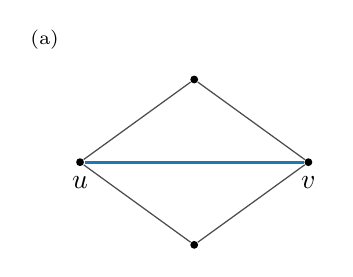
\begin{tikzpicture}[baseline]
  \BaseUV
  \coordinate (m) at ($(u)!0.5!(v)$);
  \node[v] (c1) at ($(m)+(0, 1.05)$) {};
  \node[v] (c2) at ($(m)+(0,-1.05)$) {};
  \draw[thin] (u)--(c1)--(v) (u)--(c2)--(v);
  \node[tag] at ($(u)+(-0.45,1.55)$) {{\rm (a)}};
\end{tikzpicture}
\hspace{1.2em}
% ------- (b) Xi_uv: endpoints of cross edges -------
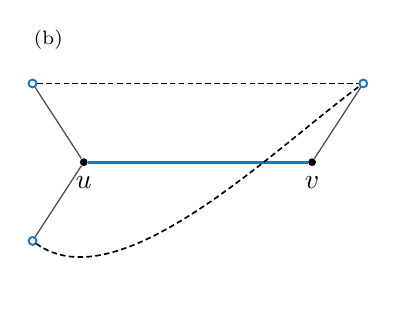
\begin{tikzpicture}[baseline]
  \BaseUV
  \node[v]    (k1) at ($(u)+(-0.65,  1.00)$) {};
  \node[v]    (k2) at ($(u)+(-0.65, -1.00)$) {};
  \node[v]    (w1) at ($(v)+( 0.65,  1.00)$) {};
  \draw[thin] (u)--(k1) (u)--(k2) (v)--(w1);

  \draw[cross] (k1) .. controls ($(k1)+(0.90, 0.00)$) and ($(w1)+(-0.90, 0.00)$) .. (w1);
  \draw[cross] (k2) .. controls ($(k2)+(1.10,-0.80)$) and ($(w1)+(-1.10,-0.80)$) .. (w1);

  \node[ring] at (k1) {};
  \node[ring] at (k2) {};
  \node[ring] at (w1) {};
  \node[tag]  at ($(u)+(-0.45,1.55)$) {{\rm (b)}};
\end{tikzpicture}
\hspace{1.2em}
% ------- (c) \widetilde\Box(k,u,v) -------
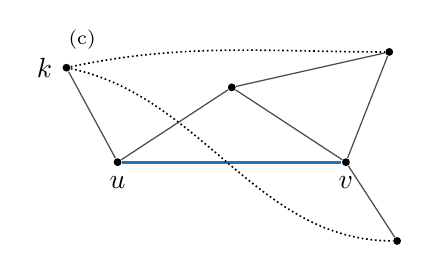
\begin{tikzpicture}[baseline]
  \BaseUV
  \coordinate (m) at ($(u)!0.5!(v)$);

  \node[v,label=left:$k$] (k)  at ($(u)+(-0.65, 1.20)$) {};

  \node[v]                (w1) at ($(v)+( 0.55,  1.40)$) {};
  \node[v]                (w2) at ($(v)+( 0.65, -1.00)$) {};

  \node[v]                (c1) at ($(m)+(0,0.95)$) {};

  \draw[thin]
    (u)--(k)
    (v)--(w1)
    (v)--(w2)
    (u)--(c1)
    (v)--(c1)

    (c1)--(w1);


  \draw[close,shorten <= 0pt,shorten >= 0pt]
       (k) to[out=12,in=180,looseness=0.95] (w1);
  \draw[close,shorten <= 0pt,shorten >= 0pt]
       (k) to[out=-12,in=180,looseness=0.95] (w2);

  \node[tag]  at ($(u)+(-0.45,1.55)$) {{\rm (c)}};
\end{tikzpicture}


\caption{
(a) \(\triangle(u,v)=|\mathcal N(u)\cap\mathcal N(v)|\);
(b) \(\Xi_{uv}\) counts \emph{vertices} in \(\mathcal U_u\cup\mathcal U_v\) that are incident to at least one cross edge: the dashed cross edges (with ring-marked \emph{vertices}) are counted;
(c) For a chosen \(k\in\mathcal N(u)\setminus\{v\}\), dotted edges indicate contributions to \(\widetilde\Box(k,u,v)\); maximizing over $k$ shows the contribution of \(\varpi_{\max}(u,v)\).}
\label{fig:local-summaries}
\end{figure}



\begin{definition}[Edge-Curvature Maps]
We consider two discrete Ricci curvatures:
\begin{align}
\mathfrak c_{\mathrm{BF}}(u,v)
&= \left(\mathfrak S(i,j)+\mathfrak T(i,j)\,\triangle(i,j)+\mathfrak C_4(i,j)\right)\mathds{1}_{\{\varrho_{\min}>1\}}
\label{eq:BF-lower-decomp}
\\[5pt]
\mathfrak c_{\mathrm{OR}}(u,v)
&=1-W_1\!\bigl(m_u,m_v\bigr),
\label{eq:cOR}
\end{align}
c.f. \citet[Definition~1]{topping_squashing_2022}, \citet[Definition~3]{ollivier_ricci_2009}.
\end{definition}


\begin{lemma}[Degree-Based Upper Bound for $\mathfrak C_4(G)$] 
\label{lem:C4-degree-only} 
For every edge $(u,v)$, 
\begin{equation} 
\label{eq:c4-edge-degree}
\frac{\Xi_{uv}}{\sho_{\max}(u,v)} \ \le\ \frac{\varrho_u+\varrho_v-2}{\max\{\varrho_u,\varrho_v\}}, 
\end{equation} 
and hence 
\begin{equation} 
\label{eq:c4-global-degree} 
\mathfrak C_4(G) \ \le\ \max_{(u,v)\in E}\ \frac{\varrho_u+\varrho_v-2}{\max\{\varrho_u,\varrho_v\}} \ \le\ 2-\frac{2}{\displaystyle\max_{v\in V}\varrho_{v}}. 
\end{equation} 
\end{lemma} 

\begin{corollary}[Structural Bound for $\Xi_{uv}$]
By \eqref{eq:c4-edge-degree} we have
\begin{equation}
\label{eq:Xi-max-structural-sharp}
\Xi_{uv} \;\leq\; \varrho_u + \varrho_v - 2 - 2\,\triangle(u,v).
\end{equation}
\end{corollary}

\begin{lemma}[Box-Count Bound]
\label{lem:box_count}
For every edge $(i,j)$, the following inequality holds:
\begin{equation}
\label{eq:sho-star}
\sho_{\max}(i,j)\ \le\ \varrho_{\max}\,(\varrho_{\max}-1)=:\sho^\star_{\max}.
\end{equation}
\end{lemma}



\section{Edgewise Bounds for \texorpdfstring{$\mathfrak c_{\rm OR}$}{cOR}}
\label{sec:edge-bound-or}

We now proceed in our analysis in two steps:
\begin{itemize}
\item[(i)] Proposition~\ref{prop:lazy-envelope-sharpened} fixes an optimal $\pi^\star$ that saturates the diagonal on $\{i,j\}\cup\mathcal C$, providing the basis for a \emph{coverage envelope} (which allows a lower bound $\mathfrak c_{\rm OR}(i,j)\ge \vartheta$ to force a necessary triangle count via $t_{\min}(\vartheta)$).

\item[(ii)] Theorem~\ref{thm:JL-plus-squares} strengthens the \citeauthor{jost_clustering_2014} bound by incorporating a matching statistic on the cross-edge bipartite graph $B_{ij}=(\mathcal U_i,\mathcal U_j;E(\mathcal U_i,\mathcal U_j))$, and Corollary~\ref{cor:JL-plus-squares-lazy} transfers this estimate to the lazy setting via the inequality of Proposition~\ref{prop:sharper-transfer}.
\end{itemize}
These results are thus the basic tools used in the next section to construct explicit \emph{upper} and \emph{lower} transfer moduli between $\mathfrak c_{\rm BF}$ and $\mathfrak c_{\rm OR}$. 

Recall that $\alpha_i\in[0,1]$ is the ``stay-put'' probability at $i$, 
$\varrho_i=\deg(i)$, and $\triangle(i,j)=|\mathcal C|$ counts common neighbors of $i$ and $j$, and that
\begin{itemize}
\item[{\rm (a)}] $w^{(\alpha)}_i,w^{(\alpha)}_j$, $w^{(\alpha)}_\wedge$ control how much mass can be shipped out of the unique neighborhoods $\mathcal U_i,\mathcal U_j$ and through the triangle channel $\mathcal C$.


\item[{\rm(b)}] $\displaystyle\Sigma^{(\alpha)}_{i,j}=\frac{\varrho_i}{1-\alpha_i}+\frac{\varrho_j}{1-\alpha_j}$ sums the inverse  of $w^{(\alpha)}_i,w^{(\alpha)}_j$ and is used in \eqref{eq:mUU-envelope-sharp}.


\item[{\rm(c)}] $z_i,z_j$ quantify how much diagonal mass can be absorbed at $i$ or $j$ when we saturate
the diagonal on $\{i,j\}\cup\mathcal C$, limiting how much must be transported out of the endpoints.
\item[{\rm(d)}] $r_i,\bar r_i,r_j,\bar r_j$ \emph{(residuals and co-residuals)} measure the imbalance between endpoint laziness and the
opposite side’s per-neighbor availability 
These terms contribute to the constant part of the envelope bound after all supply-capacity constraints are imposed.
\end{itemize}



\begin{proposition}[Lazy to Non-Lazy $\mathfrak c_{\rm OR}$ Transfer Inequality]
\label{prop:sharper-transfer}
Fix $(i,j)\in E$, and define the non-lazy OR curvature
\(
\mathfrak c_{\mathrm{OR}-0}(i,j) \;:=\; 1 - W_1(\nu_i,\nu_j).
\)
Let $\alpha_{\min}:=\min\{\alpha_i,\alpha_j\}$, $\alpha_{\max}:=\max\{\alpha_i,\alpha_j\}$, $\Delta_{ij}(\alpha):=\alpha_{\max}-\alpha_{\min}$, then for every $\beta\in[0,1]$,
\begin{equation}
\label{eq:master-beta}
\mathfrak c_{\mathrm{OR}}(i,j)
\;\ge\;
(1-\beta)\,\mathfrak c_{\mathrm{OR}-0}(i,j)\;-\;\bigl(|\alpha_i-\beta|+|\alpha_j-\beta|\bigr).
\end{equation}
In particular, with the piecewise choice
\(\alpha_\star =\alpha_{\min}\mathds 1_{\{\mathfrak c_{\mathrm{OR}\!-\!0}(i,j)\ge 0\}}+\alpha_{\max}\mathds 1_{\{\mathfrak c_{\mathrm{OR}\!-\!0}(i,j)\le 0\}}
\)
one has the bound
\begin{equation}
\label{eq:sharper-piecewise}
\mathfrak c_{\mathrm{OR}}(i,j)
\;\ge\;
(1-\alpha_\star)\,\mathfrak c_{\mathrm{OR}-0}(i,j)\;-\;\Delta_{ij}(\alpha).
\end{equation}
\end{proposition}

\begin{remark}
If $\mathfrak c_{\mathrm{OR}-0}(i,j)=0$, any $\beta\in[\alpha_{\min},\alpha_{\max}]$ yields $\mathfrak c_{\mathrm{OR}}(i,j)\ge-\Delta_{ij}(\alpha)$.
\end{remark}

In practice, the sign of $\mathfrak c_{\rm OR-0}(i,j)$ is not known \emph{a priori}, and thus for applications where $\mathfrak c_{\mathrm{OR}-0}$ is unavailable, Corollary~\ref{cor:symm-bound}~{\rm(ii)} is used instead. 

\begin{corollary}[Symmetric and General Bounds]
\label{cor:symm-bound} 
{\rm (i)} If $\alpha_i=\alpha_j=\alpha$, then $\Delta_{ij}(\alpha)=0$ and
\(\mathfrak c_{\mathrm{OR}}(i,j)\ge (1-\alpha)\,\mathfrak c_{\mathrm{OR}\!-\!0}(i,j).
\)
{\rm (ii)} If one wants a sign-agnostic bound, taking $\beta=\alpha_{\min}$ in \eqref{eq:master-beta} yields
\(
\mathfrak c_{\mathrm{OR}}(i,j)\ge (1-\alpha_{\min})\,\mathfrak c_{\mathrm{OR}\!-\!0}(i,j)-\Delta_{ij}(\alpha).
\)
\end{corollary}

\begin{proposition}[Lazy Transport Envelope for $\mathfrak c_{\mathrm{OR}}$]
\label{prop:lazy-envelope-sharpened}
Let $(i,j)\in E$ and let $\pi^\star$ be an optimal coupling between $m_i$ and $m_j$ that saturates the diagonal on $\{i,j\}\cup\mathcal C$. Define
\(
m^{(d)}:=\pi^\star\{(x,y):\mathrm{dist}_G(x,y)=d\}
\),
with $d\in\{0,1,\ge 2\}$, and decompose $m^{(1)}$ as\newline
\(
m^{(1)}=m^{(1)-\mathrm{end}} + m^{(1)-\mathrm{UU}} + m^{(1)-\triangle} + m^{(1)-\mathrm{CC}},
\)
where 
\begin{itemize}
\item[{\rm (i)}] $m^{(1)-\mathrm{end}}$ is the $\pi^\star$-mass transported along edges incident to at least one endpoint,
\item[{\rm (ii)}] $m^{(1)-\mathrm{UU}}$ is the $\pi^\star$-mass transported along cross-edges between $\mathcal U_i$ and $\mathcal U_j$,
\item[{\rm (iii)}] $m^{(1)-\triangle}$ is the $\pi^\star$-mass transported along edges between a unique and a common neighbor,
\item[{\rm (iv)}] $m^{(1)-\mathrm{CC}}$ is the $\pi^\star$-mass transported along edges internal to $\mathcal C$. 
\end{itemize}
Then the Ollivier curvature on $(i,j)$ satisfies
\begin{equation}
\label{eq:OR-master-corrected-sharp}
\mathfrak c_{\mathrm{OR}}(i,j)
\le
-1+2(z_i+z_j)
+(r_i+\bar r_i+r_j+\bar r_j)
+2\triangle(i,j)w^{(\alpha)}_\wedge
+m^{(\alpha)}_{\mathrm{UU}}
+m^{(\alpha)}_{\triangle},
\end{equation}
where the slack variables $m^{(\alpha)}_{\mathrm{UU}},m^{(\alpha)}_{\triangle}\ge 0$ may be chosen so that the following \emph{two-sided} bounds hold simultaneously:
\begin{align}
\label{eq:mUU-envelope-sharp}
m^{(1)-\mathrm{UU}}
\ &\le\ 
m^{(\alpha)}_{\mathrm{UU}}
\ \le\
\min\!\left\{
\bigl(\varrho_i-1-\triangle(i,j)\bigr)\,w^{(\alpha)}_i,
\bigl(\varrho_j-1-\triangle(i,j)\bigr)\,w^{(\alpha)}_j,
\frac{\Xi_{ij}}{\ \Sigma^{(\alpha)}_{i,j}}
\right\},
\\[4pt]
\label{eq:mTriangle-envelope-sharp}
m^{(1)-\triangle}
\ &\le\ 
m^{(\alpha)}_{\triangle}
\ \le\
\min\!\left\{
\triangle(i,j)\,\bigl|w^{(\alpha)}_i-w^{(\alpha)}_j\bigr|\ ,\ 
|\mathcal U_i|\,w^{(\alpha)}_i+|\mathcal U_j|\,w^{(\alpha)}_j
\right\}.
\end{align}
\end{proposition}



\begin{theorem}[Quadrangle-Augmented \citeauthor{jost_clustering_2014} Lower Bound]
\label{thm:JL-plus-squares}
Fix $(i,j)\!\in\! E$ and form the bipartite \emph{cross-edge graph} $
B_{ij}:=\bigl(\mathcal U_i, \mathcal U_j; E(\mathcal U_i,\mathcal U_j)\bigr),$ where $E(\mathcal U_i,\mathcal U_j):=\{(u,w)\in E:\ u\in\mathcal U_i,\ w\in\mathcal U_j\}.
$
Let $\mathfrak m(i,j)$ be the cardinality of a maximum matching in $B_{ij}$ and set
\(
\mathscr S(i,j):={\mathfrak m(i,j)}/{\max\{\varrho_i,\varrho_j\}}.
\)
Then for the non-lazy, neighbor-uniform measures $\nu_i,\nu_j$,
\begin{equation}
\label{eq:JL-aug}
\mathfrak c_{\mathrm{OR}-0}(i,j)\! \ge\!
-\Bigl[\mathfrak K(i,j)-\mathfrak Z_{\max}^{(i,j)}-\mathscr S(i,j)\Bigr]_+\!\!\!
-\Bigl[\mathfrak K(i,j)-\mathfrak Z_{\min}^{(i,j)}-\mathscr S(i,j)\Bigr]_+
\!\!\!+\mathfrak Z_{\max}^{(i,j)}.
\end{equation}
In the extremal case $\mathfrak m(i,j)=0$, this reduces to the \citet[Theorem 1, Equation (1.2)]{jost_clustering_2014} bound and, moreover, \eqref{eq:JL-aug} is monotone nondecreasing in $\mathscr S(i,j)$.
\end{theorem}

\begin{corollary}[Lazy Extension via Proposition~\ref{prop:sharper-transfer}]
\label{cor:JL-plus-squares-lazy}
With the notation of Proposition \ref{prop:sharper-transfer}, we have
\begin{multline}
\label{eq:cOR-tri-quad-bound}
\mathfrak c_{\mathrm{OR}}(i,j) \ge
(1-\alpha_\star)\Bigl(
-\bigl[\mathfrak K(i,j)-\mathfrak Z^{(i,j)}_{\max}-\mathscr S(i,j)\bigr]_+\\
-\bigl[\mathfrak K(i,j)-\mathfrak Z^{(i,j)}_{\min}-\mathscr S(i,j)\bigr]_+
+\mathfrak Z_{\max}^{(i,j)}
\Bigr) - \Delta_{ij}(\alpha).
\end{multline}
\end{corollary}

\begin{remark}
A matching-based non-lazy lower bound closely related to our $\mathscr S(i,j)$ already appears in \citet[Theorem~5.1]{bhattacharya_exact_2020}, stated in terms of a maximum matching in the ``core neighborhood'' subgraph; however \eqref{eq:JL-aug} integrates this matching capacity directly into the \citeauthor{jost_clustering_2014} framework, subtracting the normalized matching term inside the positive parts rather than applying a global linear adjustment. This decomposition isolates the precise contributions of degree imbalance, triangle overlap, and 4-cycle witnesses, enabling the translation to the localized components of $\mathfrak{c}_{\mathrm{BF}}$.
\end{remark}


\begin{remark}[Coarse $\mathfrak C_4$ Improvement]
\label{rem:coarse-C4}
If $\Xi_{ij}>0$ (which implies that $\mathfrak m(i,j)\ge 1$ and $\mathscr S(i,j)\ge \varrho_{\max}^{-1}$), then we have a uniform $\mathcal O(\varrho_{\max}^{-1})$ improvement over the triangle-only bound.
\end{remark}


\begin{proposition}[Monotone Coverage Envelope for $\mathfrak c_{\mathrm{OR}}$]
\label{prop:coverage-envelope-monotone}
Let $(i,j)\in E$, and define the intercept and slope
\begin{equation}
\label{eq:const-slope}
\begin{aligned}
\mathrm{Const}_\alpha
&:=
-1+2(z_i+z_j)
+(r_i+\bar r_i+r_j+\bar r_j)
+\frac{\varrho_i+\varrho_j-2}{\Sigma^{(\alpha)}_{i,j}},
\\
\mathrm{Slope}_\alpha
&:=w^{(\alpha)}_i+w^{(\alpha)}_j-\frac{2}{\Sigma^{(\alpha)}_{i,j}}.
\end{aligned}
\end{equation}
Then for every $\triangle(i,j)\in[0,\varrho_{\min}-1]$,
\begin{equation}
\label{eq:Theta-alpha-def}
\mathfrak c_{\mathrm{OR}}(i,j)\ \le\ 
\Theta_\alpha(\triangle(i,j))\ :=\ \mathrm{Const}_\alpha+\mathrm{Slope}_\alpha\triangle(i,j),
\end{equation}
and $\Theta_\alpha$ is affine and non-decreasing on $[0,\varrho_{\min}-1]$.
\end{proposition}


\section{Transfer Principles Between \texorpdfstring{$\mathfrak c_{\rm OR}$}{cOR} and \texorpdfstring{$\mathfrak c_{\rm BF}$}{cBF}}
\label{sec:transfer-curvatures}
The central idea is to decouple \emph{structure} from \emph{transport}: using the results of Section~\ref{sec:edge-bound-or}, we obtain closed-form, monotone, piecewise-affine moduli that depend solely on the combinatoric summaries around \((i,j)\).

We establish four transfer principles:
\begin{itemize}

\item[(i)]  
Given a target BF level \(\zeta\), we determine the minimum triangle mass \(\mathscr Z^{(i,j)}(\zeta)\), which, together with a square-matching floor, yields an explicit modulus \(\varphi^{(i,j)}_{\rm BF\to OR}(\zeta)\) with
\[
\mathfrak c_{\rm BF}(i,j)\ge \zeta 
\implies
\mathfrak c_{\rm OR}(i,j)\ge \varphi^{(i,j)}_{\rm BF\to OR}(\zeta).
\]

\item[(ii)]  
Interpreting the constraint \(\mathfrak c_{\mathrm{BF}}\le \zeta\) as a budget on the unit-cost operations that increase \(\mathfrak c_{\mathrm{OR}}\), we obtain simultaneous bounds on triangle mass and cross-edges,
\[
0 \le \triangle \le \triangle_{\max}(\zeta), \qquad
0 \le \Xi_{ij} \le \Xi_{\max}(\triangle),
\]
which induce a continuous, piecewise-affine function \(\widehat{\Psi}_\alpha(\triangle)\) whose maximizer, lying in the finite knot set~\eqref{eq:knot-set}, yields the upper modulus
\[
\mathfrak c_{\mathrm{OR}}(i,j) \le \psi^{(i,j)}_{\mathrm{BF}\to \mathrm{OR}}(\zeta).
\]


\item[(iii)]  
The coverage envelope \(\Theta_\alpha(\triangle)\) is invertible: observing \(\mathfrak c_{\rm OR}\ge \vartheta\) enforces at least \(t_{\min}(\vartheta)\) shared neighbors.  
Using this guaranteed overlap and discarding the nonnegative $4$-cycle term gives the lower bound
\[
\mathfrak c_{\rm BF}(i,j)\ \ge\ \mathfrak S(i,j)+\mathfrak T(i,j)\,t_{\min}(\vartheta).
\]

\item[(iv)]  
Combining the lazy to non-lazy reduction with a quadrangle-effective deficit \(\mathfrak K_\square\) (which penalizes degrees via the matching statistic), we construct a piecewise-affine triangle envelope \(\mathfrak u_{\max}^{(i,j)}(\vartheta)\).  
Substituting into \(\mathfrak c_{\rm BF}\) yields
\[
\mathfrak c_{\rm OR}(i,j)\le \vartheta
\implies
\mathfrak c_{\rm BF}(i,j)
\ \le\ 
\mathfrak S(i,j)+\mathfrak T(i,j)\,\mathfrak u_{\max}^{(i,j)}(\vartheta)+\mathfrak C_4(i,j).
\]

\end{itemize}
Together, these moduli (a) provide computable curvature intervals using only local combinatorics, (b) isolate the precise roles of degree imbalance, triangle overlap, and coarse $4$-cycle evidence, (c) work directly in the lazy setting with explicit dependence on \((\alpha_i,\alpha_j)\), and (d) avoid any optimal transport computation.  
They enable fast screening (e.g.\ certifying the sign or a prescribed threshold of one curvature from the other), offer interpretable sensitivity to local edits (e.g.\ effects of adding a triangle or cross-edge), and support structural inference: large OR curvature forces a minimum triangle count through \(t_{\min}\), while a BF budget imposes strict limits on how unique-unique and unique-common mass can increase \(\mathfrak c_{\rm OR}\).  
The piecewise-affine form also makes these envelopes amenable to optimization and embedding procedures in which curvature appears as a constraint or regularizer.

\begin{theorem}[$\mathfrak c_{\rm BF}$ to $\mathfrak c_{\rm OR}$ Lower Transfer Modulus]
\label{thm:bf-to-or}
Fix $(i,j)\in E$ and define
\[
\mathscr Z^{(i,j)}(\zeta)\ :=\ \max\!\left\{0,\ \frac{\,\zeta-\mathfrak S(i,j)-\mathfrak C_4(i,j)\,}{\mathfrak T(i,j)}\right\},
\]
as well as
\[
\overline{\mathscr Z}^{(i,j)}_{\bullet}(\zeta)\ :=\ \frac{\mathscr Z^{(i,j)}(\zeta)}{\bullet\{\varrho_i,\varrho_j\}},\qquad \ \bullet\in\{\min,\max\},
\]
and the square-matching floor
\begin{equation}
\label{eq:S-underline-rigorous}
\underline{\mathscr S}^{(i,j)}(\zeta)
\ :=\
\max\left\{\ \frac12\,\mathfrak C_4(i,j),\ \ \frac12\,\left[\zeta-\mathfrak S(i,j)-\mathfrak T(i,j)\,(\varrho_{\min}-1)\,\right]_+\ \right\}.
\end{equation}
Set the non-lazy transfer modulus
\begin{equation}
\label{eq:phi-nonlazy-square-rigorous}
\begin{aligned}
\varphi^{(i,j)}_{\rm BF\to OR-0}(\zeta)
&:=
-\Bigl[\mathfrak K(i,j)-\overline{\mathscr Z}^{(i,j)}_{\max}(\zeta)-\underline{\mathscr S}^{(i,j)}(\zeta)\Bigr]_+\\
&\quad
-\Bigl[\mathfrak K(i,j)-\overline{\mathscr Z}^{(i,j)}_{\min}(\zeta)-\underline{\mathscr S}^{(i,j)}(\zeta)\Bigr]_+
\ +\ \overline{\mathscr Z}^{(i,j)}_{\max}(\zeta),
\end{aligned}
\end{equation}
and its lazy counterpart via Corollary~\ref{cor:JL-plus-squares-lazy},
\begin{equation}
\label{eq:phi-lazy-square-rigorous}
\varphi^{(i,j)}_{\rm BF\to OR}(\zeta)
\ :=\ (1-\alpha_\star)\,\varphi^{(i,j)}_{\rm BF\to OR-0}(\zeta)\ -\ \Delta_{ij}(\alpha),
\end{equation}
where $\alpha_\star$ is the piecewise choice in Proposition~\ref{prop:sharper-transfer}. Then, for every $\zeta\in\mathbb R$,
\[
\mathfrak c_{\rm BF}(i,j)\ \ge\ \zeta\ \implies\ \mathfrak c_{\rm OR}(i,j)\ \ge\ \varphi^{(i,j)}_{\rm BF\to OR}(\zeta).
\]
\end{theorem}


\begin{theorem}[$\mathfrak c_{\rm BF}$ to $\mathfrak c_{\rm OR}$ Upper Transfer Modulus]
\label{thm:BF-to-OR-lazy}
Fix an edge $(i,j)\in E$, assume $\mathfrak c_{\rm BF}(i,j)\le \zeta$ for some $\zeta\in\mathbb R$ and set
\(
\mathscr b(\zeta)\ :=\ [\,\zeta-\mathfrak S(i,j)\,]_+.
\)
The following inequalities follow
\begin{equation}
\label{eq:bf-budget-region}
\begin{aligned}
0 & \le \triangle(i,j) \le\ \triangle_{\max}(i,j):=\min\!\left\{\varrho_{\min}-1,\ \frac{\mathscr b(\zeta)}{\mathfrak T(i,j)}\right\},
\\
0 & \le \Xi_{ij} \le\ \Xi_{\max}\left(\triangle(i,j)\right),
\end{aligned}
\end{equation}
where
\begin{equation}
\label{eq:Xi-upper-two-sources}
\begin{aligned}
\Xi_{\max}(\triangle) & :=\ \min\!\left\{
\underbrace{\sho_{\max}^\star\Bigl(\mathscr b(\zeta)-\mathfrak T(i,j)\triangle\Bigr)_+}_{\text{\rm Lemma \ref{lem:box_count}}},
\ \underbrace{\ \varrho_i+\varrho_j-2-2\triangle\ }_{\text{\rm Equation \eqref{eq:Xi-max-structural-sharp}}}
\right\},
\\
\sho_{\max}^\star&:=\varrho_{\max}(\varrho_{\max}-1).
\end{aligned}
\end{equation}
Define the affine functions in the triangle variable $\triangle$:
\begin{align}
\label{eq:Amin}
A_u(\triangle)&:=(\varrho_u-1-\triangle)\,w^{(\alpha)}_u,\qquad
A_{\min}(\triangle):=\min\{A_i(\triangle),A_j(\triangle)\},\\[3pt]
\label{eq:Balph}
B_\alpha(\triangle)&:=\frac{\sho_{\max}^\star}{\Sigma^{(\alpha)}_{i,j}}\,\Bigl(\mathscr b(\zeta)-\mathfrak T(i,j)\triangle\Bigr),\\[3pt]
\label{eq:Dalph}
D_\alpha(\triangle)&:=\frac{\varrho_i+\varrho_j-2-2\triangle}{\Sigma^{(\alpha)}_{i,j}},\\[3pt]
\label{eq:Calph}
C_\alpha(\triangle)&:=\min\!\left\{\ \triangle\,\bigl|w^{(\alpha)}_i-w^{(\alpha)}_j\bigr|\,,\ A_i(\triangle)+A_j(\triangle)\ \right\}.
\end{align}
Then, with the endpoint quantities from the lazy envelope
\[
z_u=\min\!\left\{\alpha_u,\frac{1-\alpha_{u^\complement}}{\varrho_{u^\complement}}\right\},\quad
r_u:=\Bigl[\alpha_u-\frac{1-\alpha_{u^\complement}}{\varrho_{u^\complement}}\Bigr]_+,\quad
\bar r_u:=\Bigl[\frac{1-\alpha_{u^\complement}}{\varrho_{u^\complement}}-\alpha_u\Bigr]_+,
\]
we have the piecewise-affine upper envelope
\begin{multline}
\label{eq:widehat-Psi}
\widehat\Psi_\alpha(\triangle)
:=
-1+2(z_i+z_j)
+\bigl(r_i+\bar r_i+r_j+\bar r_j\bigr)
+2\,w^{(\alpha)}_\wedge\,\triangle \\
+\Bigl[\min\{A_{\min}(\triangle),\,B_\alpha(\triangle),\,D_\alpha(\triangle)\}\Bigr]_+
+C_\alpha(\triangle).
\end{multline}
Consequently,
\begin{equation}
\label{eq:BF-to-OR-claim-sharp}
\mathfrak c_{\rm OR}(i,j)
\ \le\
\psi_{\rm BF\to OR}^{(i,j)}(\zeta)
:=\max_{\ \triangle\in[\,0,\ \triangle_{\max}(i,j)\,]}\ \widehat\Psi_\alpha(\triangle).
\end{equation}

\noindent
Moreover, $\widehat\Psi_\alpha$ is continuous and piecewise-affine on $[0,\triangle_{\max}(i,j)]$, and any maximizer in \eqref{eq:BF-to-OR-claim-sharp} can be chosen from the finite set
\begin{equation}
\label{eq:knot-set}
\mathcal K := \Bigl\{0, \triangle_{\max}, \triangle_{\rm swap}, \triangle_{i\cap B}, \triangle_{j\cap B}, \triangle_{i\cap D}, \triangle_{j\cap D}, \triangle_{B\cap D}, \triangle_{\mathscr s\cap}\Bigr\} \cap [0,\triangle_{\max}],
\end{equation}
where
\[
\begin{aligned}
\triangle_{\rm swap}&:=\begin{cases}
\displaystyle\frac{w^{(\alpha)}_j(\varrho_j-1)-w^{(\alpha)}_i(\varrho_i-1)}{\,w^{(\alpha)}_j-w^{(\alpha)}_i\,},&\text{if }w^{(\alpha)}_i\neq w^{(\alpha)}_j,\\[8pt]
\text{Undefined},&\text{if }w^{(\alpha)}_i= w^{(\alpha)}_j,
\end{cases}\\[6pt]
\triangle_{u\cap B}&:=\ \frac{\ \dfrac{\sho_{\max}^\star}{\Sigma^{(\alpha)}_{i,j}}\,\mathscr b(\zeta)\ -\ w^{(\alpha)}_u(\varrho_u-1)\ }{ \ \dfrac{\sho_{\max}^\star}{\Sigma^{(\alpha)}_{i,j}}\,\mathfrak T(i,j)\ -\ w^{(\alpha)}_u\ }\qquad(u\in\{i,j\})\quad\text{if the denominator is nonzero},\\[8pt]
\triangle_{u\cap D}&:=\ \frac{\ (\varrho_i+\varrho_j-2)\ -\ \Sigma^{(\alpha)}_{i,j}\,w^{(\alpha)}_u(\varrho_u-1)\ }{\,2-\Sigma^{(\alpha)}_{i,j}\,w^{(\alpha)}_u\,}\qquad(u\in\{i,j\})\quad\text{if the denominator is nonzero},\\[8pt]
\triangle_{B\cap D}&:=\ \frac{\,\varrho_i+\varrho_j-2\ -\ \sho_{\max}^\star\,\mathscr b(\zeta)\,}{\,2-\sho_{\max}^\star\,\mathfrak T(i,j)\,}\quad\text{if the denominator is nonzero},\\[8pt]
\triangle_{\mathscr s\cap}&:=\ \frac{\,w^{(\alpha)}_i(\varrho_i-1)+w^{(\alpha)}_j(\varrho_j-1)\,}{\,w^{(\alpha)}_i+w^{(\alpha)}_j+\bigl|w^{(\alpha)}_i-w^{(\alpha)}_j\bigr|\,}.
\end{aligned}
\]
\end{theorem}


\begin{theorem}[$\mathfrak c_{\rm OR}$ to $\mathfrak c_{\rm BF}$ Upper Transfer Modulus]
\label{thm:OR-to-BF-lower}
Let $(i,j)\in E$ with $\varrho_{\min}\ge 2$. For any $\vartheta\in\mathbb R$, define
\begin{equation}\label{eq:tmin}
t_{\min}(\vartheta):=\min \left\{ \left[\frac{\ \vartheta-\mathrm{Const}_\alpha\ }{\ \mathrm{Slope}_\alpha\ }\right]_+,\ \left(\varrho_{\min}-1\right)\right\},
\end{equation}
with $\mathrm{Const}_\alpha,\mathrm{Slope}_\alpha$ from \eqref{eq:const-slope}. Then
\begin{equation}\label{eq:OR-to-BF-lower}
\mathfrak c_{\rm OR}(i,j)\ \ge\ \vartheta
\implies
\mathfrak c_{\rm BF}(i,j)\ \ge\ \varphi_{\rm OR\to BF}^{(i,j)}(\vartheta):=\ \mathfrak S(i,j)+\mathfrak T(i,j)\,t_{\min}(\vartheta).
\end{equation}
Moreover,
\begin{itemize}
\item[{\rm (a)}] If $\vartheta\le \mathrm{Const}_\alpha$, then \eqref{eq:OR-to-BF-lower} reduces to the degree-only bound $\mathfrak c_{\rm BF}\ge \mathfrak S(i,j)$.
\item[{\rm (b)}] If $\vartheta>\Theta_\alpha(\varrho_{\min}-1)$ (with $\Theta_\alpha$ as in \eqref{eq:Theta-alpha-def}), then no edge with the given $(\varrho_i,\varrho_j,\alpha_i,\alpha_j)$ can satisfy $\mathfrak c_{\rm OR}\ge\vartheta$; thus the implication is vacuous.
\item[{\rm (c)}] The modulus $\varphi^{(i,j)}_{\rm OR\to BF}$ depends only on $(\varrho_i,\varrho_j,\alpha_i,\alpha_j)$ and is independent of $\Xi_{ij}$ and other higher-order edge substructures as \eqref{eq:Theta-alpha-def} uses only the structural bound \eqref{eq:Xi-max-structural-sharp}.
\end{itemize}
\end{theorem}


\begin{theorem}[$\mathfrak c_{\rm OR}$ to $\mathfrak c_{\rm BF}$ Upper Transfer Modulus]
\label{thm:or-to-bf}
Let $(i,j)\in E$ and define the
\(
\mathfrak s_0^{(i,j)}(\vartheta) := {(\vartheta+\Delta_{ij}(\alpha))}/{(1-\alpha_\star)}.
\)
Set the deficit
\(
\mathfrak K_{\square}(i,j) :=\bigl[\mathfrak K(i,j)-\mathscr S(i,j)\bigr]_+
\)
and the corresponding breakpoint value
\(
\mathfrak s_{\mathfrak u}^{\square}(i,j)\ :=\ \mathfrak K_{\square}(i,j)\,\Bigl(2\,{\varrho_{\min}}/{\varrho_{\max}}-1\Bigr).
\)
Define the piecewise \emph{quadrangle triangle-envelope}
\begin{equation}
\label{eq:u-max-square}
\mathfrak u_{\max}^{(i,j)}(\vartheta)\ :=\
\begin{cases}
0,
& \mathfrak s_0^{(i,j)}(\vartheta)\le -2\,\mathfrak K_{\square}(i,j),\\[8pt]
\dfrac{\mathfrak s_0^{(i,j)}(\vartheta)+2\,\mathfrak K_{\square}(i,j)}{\ \mathfrak T(i,j)\ },
& -2\,\mathfrak K_{\square}(i,j)\le \mathfrak s_0^{(i,j)}(\vartheta)\le \mathfrak s_{\mathfrak u}^{\square}(i,j),\\[12pt]
\dfrac{\varrho_{\max}}{2}\,\Bigl(\mathfrak s_0^{(i,j)}(\vartheta)+\mathfrak K_{\square}(i,j)\Bigr),
& \mathfrak s_{\mathfrak u}^{\square}(i,j)\le \mathfrak s_0^{(i,j)}(\vartheta)\le \mathfrak K_{\square}(i,j),\\[12pt]
\varrho_{\max}\,\mathfrak s_0^{(i,j)}(\vartheta),
& \mathfrak s_0^{(i,j)}(\vartheta)\ge \mathfrak K_{\square}(i,j).
\end{cases}
\end{equation}
Finally, set the \emph{quadrangle-augmented lazy modulus}
\begin{equation}
\label{eq:psi-square}
\psi^{(i,j)}_{\rm OR\to BF}(\vartheta)
\ :=\ \mathfrak S(i,j)\ +\ \mathfrak T(i,j)\,\mathfrak u_{\max}^{(i,j)}(\vartheta)\ +\ \mathfrak C_4(i,j).
\end{equation}
Then the following implication holds:
\(
\mathfrak c_{\rm OR}(i,j) \le \vartheta
\implies
\mathfrak c_{\rm BF}(i,j) \le\psi^{(i,j)}_{\rm OR\to BF}(\vartheta).
\)
\end{theorem}



\section{Analytical Results}
\label{sec:analysis}
\begin{figure}
\centering
\includegraphics[width=0.8\linewidth]{figures_paper/runtime_scaling_loglog_neurips.pdf}
\caption{\textbf{Empirical Runtime Scaling.} Log-log comparison of execution time for exact $\mathfrak c_{\rm OR}$ versus the proposed transfer moduli on Erd\H{o}s--R\'enyi graphs ($n \in [50, 15{,}000]$). In addition to the divergence in scaling exponents (slopes), the exact computation sits two orders of magnitude higher in absolute runtime.}
\label{fig:runtime_scaling}
\end{figure}

We now seek to provide experimental confirmation for the two families of edgewise bounds derived above: the \emph{coverage envelope} for $\mathfrak c_{\rm OR}$ (Proposition~\ref{prop:coverage-envelope-monotone}) and the \emph{transfer inequalities} between $\mathfrak c_{\rm OR}$ and $\mathfrak c_{\rm BF}$ (Theorems~\ref{thm:OR-to-BF-lower} and~\ref{thm:bf-to-or}). To evaluate both the computational scalability and the tightness of our transfer moduli, we benchmark across a comprehensive suite of synthetic topologies and empirical networks (Karate, Jazz, Power Grid, Yeast, HepPh); complete generation parameters and structural descriptions are deferred to Appendix~\ref{appendix:graph-gen}.

\paragraph{Empirical Runtime Scaling.}

Evaluating $\mathfrak c_{\rm OR}$ exactly is fundamentally bottlenecked by the underlying optimal transport solvers. Figure~\ref{fig:runtime_scaling} isolates this computational barrier: we benchmarked total edgewise execution times across a logarithmically spaced sequence of ER graphs ranging from $n=50$ to $n\approx15{,}000$, and to isolate topological scaling from density bloat, we let $p \propto n^{-0.6}$ be the edge probability, ensuring the average degree grew sub-linearly at $\mathcal{O}(n^{0.4})$. As shown, exact evaluation exhibits steep polynomial scaling and sits orders of magnitude higher in absolute time, rapidly becoming intractable for large networks despite highly parallelized execution. In contrast, our transfer moduli parameterize the transport cost entirely through 2-hop local combinatorics, decoupling curvature estimation from global network size, and yielding remarkable asymptotic and constant-factor speedups.


\paragraph{Summary Statistics.}
Tables~\ref{tab:bandwidth_bf2or} and~\ref{tab:bandwidth_or2bf} quantify two complementary aspects of the curvature relationships:
\begin{itemize}
    \item[(i)] \emph{Intrinsic heterogeneity:} the original bandwidths (edgewise ranges of $\mathfrak c_{\mathrm{OR}}$ and $\mathfrak c_{\mathrm{BF}}$);
    \item[(ii)] \emph{Transfer informativeness:} for each direction (BF$\!\to$OR and OR$\!\to$BF), both the \emph{transfer-band width} (Max, 95th percentile) and the \emph{slack} to the nearest transfer bound (Median, 95th percentile).
\end{itemize}


Widths are expressed in the units of the \emph{target curvature}, with smaller widths and smaller slacks indicating tighter, more informative transfer. Curvatures are edgewise constant on $K_n$, $C_n$, and the 2D tori, so $r$ is undefined and the transfer bands collapse to constants. 

\begin{table}
\centering
\caption{Summary of $\mathfrak c_{\mathrm{BF}}\!\to\!\mathfrak c_{\mathrm{OR}}$ transfer. 
We report edge counts $|E|$, correlation $r=\mathrm{corr}(\mathfrak c_{\rm OR}, \mathfrak c_{\rm BF})$, 
original (edgewise) ranges for $\mathfrak c_{\rm OR}$ and $\mathfrak c_{\rm BF}$, and the transfer-band width (Max, 95P) and slack (50P, 95P). 
Correlation is “--” if one curvature is edgewise constant.}
\label{tab:bandwidth_bf2or}
\begin{adjustbox}{max width=\textwidth}
\footnotesize
\setlength{\tabcolsep}{4pt}
\begin{tabular}{l c c r r r r r r}
\toprule
Graph & $|E|$ & $r$ & $\mathfrak c_{\rm OR}$ range & $\mathfrak c_{\rm BF}$ range & \multicolumn{2}{c}{Width} & \multicolumn{2}{c}{Slack} \\
\cmidrule(lr){6-7} \cmidrule(lr){8-9}
& & & & & Max & 95P & 50P & 95P \\
\midrule
BA(800, 2) & 1597 & 0.947 & 2.133 & 2.631 & 1.801 & 1.561 & 0.130 & 0.318 \\
BA(800, 5) & 3985 & 0.558 & 1.310 & 1.514 & 1.832 & 1.676 & 0.590 & 0.769 \\
BA(1600, 2) & 3197 & 0.961 & 2.209 & 2.672 & 1.854 & 1.548 & 0.072 & 0.278 \\
BA(1600, 5) & 7985 & 0.608 & 1.417 & 1.804 & 1.869 & 1.722 & 0.511 & 0.787 \\
K$_{120}$ & 7140 & -- & 0.000 & 0.000 & 0.017 & 0.017 & 0.000 & 0.000 \\
C$_{600}$ & 600 & -- & 0.000 & 0.000 & 0.333 & 0.333 & 0.000 & 0.000 \\
Torus(32,32) & 2048 & -- & 0.000 & 0.000 & 0.571 & 0.571 & 0.000 & 0.000 \\
Torus(40,40) & 3200 & -- & 0.000 & 0.000 & 0.571 & 0.571 & 0.000 & 0.000 \\
Grid(40,40) & 3120 & 0.998 & 0.250 & 0.333 & 0.673 & 0.644 & 0.000 & 0.200 \\
G(800, 0.010013) & 3234 & 0.741 & 1.174 & 1.200 & 1.650 & 1.507 & 0.260 & 0.412 \\
G(1600, 0.005003) & 6420 & 0.793 & 1.442 & 1.746 & 1.694 & 1.507 & 0.169 & 0.355 \\
RGG(800, 0.056419) & 2986 & 0.960 & 2.143 & 2.881 & 1.406 & 1.055 & 0.161 & 0.385 \\
RGG(1600, 0.039894) & 6119 & 0.963 & 2.352 & 2.848 & 1.435 & 1.067 & 0.165 & 0.371 \\
HRG(800, 5.0, 1.0, 0.0) & 59231 & 0.980 & 1.374 & 2.264 & 1.424 & 1.165 & 0.146 & 0.453 \\
HRG(800, 5.0, 1.0, 0.5) & 77050 & 0.869 & 0.680 & 2.044 & 1.877 & 1.533 & 0.003 & 0.006 \\
WS(800,10,0.05) & 4000 & 0.967 & 2.411 & 2.578 & 1.526 & 1.014 & 0.191 & 0.402 \\
WS(800,10,0.2) & 4000 & 0.964 & 2.333 & 2.492 & 1.589 & 1.355 & 0.269 & 0.498 \\
WS(1600,10,0.05) & 8000 & 0.967 & 2.399 & 2.575 & 1.524 & 1.007 & 0.191 & 0.402 \\
WS(1600,10,0.2) & 8000 & 0.967 & 2.441 & 2.617 & 1.576 & 1.295 & 0.237 & 0.467 \\
Jazz & 2742 & 0.912 & 1.713 & 2.877 & 1.761 & 1.279 & 0.150 & 0.446 \\
Karate & 78 & 0.866 & 1.548 & 2.396 & 1.414 & 1.229 & 0.249 & 0.533 \\
Power Grid & 6594 & 0.940 & 2.427 & 3.078 & 1.475 & 1.018 & 0.071 & 0.308 \\
Yeast & 1081 & 0.692 & 2.684 & 2.814 & 1.723 & 1.410 & 0.212 & 0.501 \\
Arxiv & 420877 & 0.759 & 2.888 & 3.476 & 1.972 & 1.807 & 0.442 & 0.787 \\
\bottomrule
\end{tabular}
\end{adjustbox}
\end{table}

Random geometric and Watts--Strogatz graphs exhibit narrow  $\mathfrak{c}_{\mathrm{BF}} \to \mathfrak{c}_{\mathrm{OR}}$ bands, whereas Erd\H{o}s--R\'enyi graphs show broader bands and reduced correlations ($r = 0.74$--$0.79$), with Barab\'asi--Albert graphs exhibiting a similar behavior as the parameter $m$ increases.

In hyperbolic random graphs, where the \emph{temperature} $T$ governs the softness of the connection probability%
\footnote{Lower $T$ produces nearly deterministic, distance-threshold connections while higher $T$  introduces randomness by flattening the distance dependence in the linking kernel.}%
, at low temperature high association is preserved ($r \approx 0.98$) with a tight transfer band, with the band broadening and additional slack being introduced as $T$ increases. 

Real networks mirror these trends: Jazz and Karate exhibit tight $\mathfrak c_{\rm BF}\!\to\!\mathfrak c_{\rm OR}$, with the Power Grid shows the tightest transfer, while Yeast and ArXiv display wide bandwidths and loose transfer.

\begin{table}
\centering
\caption{Summary of $\mathfrak c_{\mathrm{OR}}\!\to\!\mathfrak c_{\mathrm{BF}}$ transfer. 
Columns and notation as in Table~\ref{tab:bandwidth_bf2or}.}
\label{tab:bandwidth_or2bf}
\begin{adjustbox}{max width=\textwidth}
\footnotesize
\setlength{\tabcolsep}{4pt}
\begin{tabular}{l c c r r r r r r}
\toprule
Graph & $|E|$ & $r$ & $\mathfrak c_{\rm OR}$ range & $\mathfrak c_{\rm BF}$ range & \multicolumn{2}{c}{Width} & \multicolumn{2}{c}{Slack} \\
\cmidrule(lr){6-7} \cmidrule(lr){8-9}
& & & & & Max & 95P & 50P & 95P \\
\midrule
BA(800, 2) & 1597 & 0.947 & 2.133 & 2.631 & 3.333 & 0.736 & 0.000 & 0.225 \\
BA(800, 5) & 3985 & 0.558 & 1.310 & 1.514 & 1.807 & 1.323 & 0.205 & 0.453 \\
BA(1600, 2) & 3197 & 0.961 & 2.209 & 2.672 & 2.000 & 0.572 & 0.000 & 0.154 \\
BA(1600, 5) & 7985 & 0.608 & 1.417 & 1.804 & 1.664 & 1.124 & 0.150 & 0.367 \\
K$_{120}$ & 7140 & -- & 0.000 & 0.000 & 0.000 & 0.000 & 0.000 & 0.000 \\
C$_{600}$ & 600 & -- & 0.000 & 0.000 & 0.000 & 0.000 & 0.000 & 0.000 \\
Torus(32,32) & 2048 & -- & 0.000 & 0.000 & 1.000 & 1.000 & 0.000 & 0.000 \\
Torus(40,40) & 3200 & -- & 0.000 & 0.000 & 1.000 & 1.000 & 0.000 & 0.000 \\
Grid(40,40) & 3120 & 0.998 & 0.250 & 0.333 & 1.833 & 1.833 & 0.000 & 0.667 \\
G(800, 0.010013) & 3234 & 0.741 & 1.174 & 1.200 & 1.117 & 0.760 & 0.000 & 0.305 \\
G(1600, 0.005003) & 6420 & 0.793 & 1.442 & 1.746 & 0.964 & 0.559 & 0.000 & 0.200 \\
RGG(800, 0.056419) & 2986 & 0.960 & 2.143 & 2.881 & 2.167 & 1.765 & 0.200 & 0.498 \\
RGG(1600, 0.039894) & 6119 & 0.963 & 2.352 & 2.848 & 2.000 & 1.762 & 0.205 & 0.486 \\
HRG(800, 5.0, 1.0, 0.0) & 59231 & 0.980 & 1.374 & 2.264 & 1.997 & 1.844 & 0.114 & 0.687 \\
HRG(800, 5.0, 1.0, 0.5) & 77050 & 0.869 & 0.680 & 2.044 & 1.929 & 1.654 & 0.297 & 0.571 \\
WS(800,10,0.05) & 4000 & 0.967 & 2.411 & 2.578 & 1.839 & 1.800 & 0.231 & 0.457 \\
WS(800,10,0.2) & 4000 & 0.964 & 2.333 & 2.492 & 1.880 & 1.778 & 0.298 & 0.560 \\
WS(1600,10,0.05) & 8000 & 0.967 & 2.399 & 2.575 & 1.830 & 1.800 & 0.232 & 0.459 \\
WS(1600,10,0.2) & 8000 & 0.967 & 2.441 & 2.617 & 1.885 & 1.768 & 0.264 & 0.524 \\
Jazz & 2742 & 0.912 & 1.713 & 2.877 & 1.968 & 1.883 & 0.416 & 0.826 \\
Karate & 78 & 0.866 & 1.548 & 2.396 & 2.042 & 1.847 & 0.163 & 0.805 \\
Power Grid & 6594 & 0.940 & 2.427 & 3.078 & 3.333 & 1.263 & 0.000 & 0.333 \\
Yeast & 1081 & 0.692 & 2.684 & 2.814 & 3.333 & 1.238 & 0.023 & 0.402 \\
Arxiv & 420877 & 0.759 & 2.888 & 3.476 & 3.333 & 1.873 & 0.421 & 0.820 \\
\bottomrule
\end{tabular}
\end{adjustbox}
\end{table}


\paragraph{Empirical Plots across Models.} 


Figures \ref{fig:scatters}, and \ref{fig:dists_sel} visualize these dynamics. In RGGs, the scatter forms a narrow, positive-slope band where the conditional median tracks the upper transfer curve, reflecting saturated unit-cost budgets due to geometric clustering. The right tail of the $\mathfrak c_{\rm OR}$ histogram is tightly bracketed by the upper envelope, confirming that our coupling-free bounds are highly informative for one-step geometries. In sparse ER graphs, the scatter widens and shifts negative. The conditional median aligns with the lower transfer curve over most of the support, driven by scarce triangles and predominantly unique-unique flow. 


\begin{figure}
\centering
\includegraphics[width=.48\textwidth]{figures_paper/fig_scatter_cBF_cOR__er_n800_p0_0100125_2d_Hist.png}\hfill
\includegraphics[width=.48\textwidth]{figures_paper/fig_scatter_cBF_cOR__ws_n800_k10_b0_2_2d_Hist.png}

\vspace{2pt}

\includegraphics[width=.48\textwidth]{figures_paper/fig_scatter_cBF_cOR__ba_n1600_m2_2d_Hist.png}\hfill 
\includegraphics[width=.48\textwidth]{figures_paper/fig_scatter_cBF_cOR__rg_n1600_r0_039894_2d_Hist.png}

\vspace{2pt}

\includegraphics[width=.48\textwidth]{figures_paper/fig_scatter_cBF_cOR__hrg_n800_R5_0_a1_0_T0_5_2d_Hist.png}\hfill
\includegraphics[width=.48\textwidth]{figures_paper/fig_scatter_cBF_cOR__sbm2_n1000_pin0_012018_pout0_004006_2d_Hist.png}



\caption{\textbf{Representative edgewise scatter plots.}
Blue points: sampled edges; black: $\mathrm{median}[\mathfrak c_{\rm OR}\mid \mathfrak c_{\rm BF}]$; 
green (red) dash-dot: median of the \emph{lower} (\emph{upper}) transfer $\mathfrak c_{\rm BF}\mapsto\mathfrak{c}_{\rm OR}$.
Panels: ER, WS, BA, RGG, HRG, SBM (assortatitve) (left-to-right, top-to-bottom).}
\label{fig:scatters}
\end{figure}

WS graphs blend these behaviors: the conditional median tracks the lower transfer for very negative $\mathfrak c_{\rm BF}$ with a remarkable jump around the bottom quintile. BA graphs display a pronounced fan-out; hub-incident edges push $\mathfrak c_{\rm BF}$ negative (as degree penalties dominate), while $\mathfrak c_{\rm OR}$ remains comparatively less negative because optimal transport partially absorbs mass at the endpoints. Finally, in HRGs, the conditional median closely follows the upper transfer across the entire $\mathfrak c_{\rm BF}$ range, demonstrating that our analytical upper transfer is essentially tight and predictive in positively curved ambient geometries.



\begin{figure}
\centering
\includegraphics[width=.48\textwidth]{figures_paper/fig_cOR_hist__rg_n800_r0_056419.png}\hfill
\includegraphics[width=.48\textwidth]{figures_paper/fig_cBF_hist__rg_n800_r0_056419.png}

\vspace{2pt}

\includegraphics[width=.48\textwidth]{figures_paper/fig_cOR_hist__er_n800_p0_0100125.png}\hfill
\includegraphics[width=.48\textwidth]{figures_paper/fig_cBF_hist__er_n800_p0_0100125.png}

\vspace{2pt}

\includegraphics[width=.48\textwidth]{figures_paper/fig_cOR_quantile__ws_n800_k10_b0_2.png}
\hfill
\includegraphics[width=.48\textwidth]{figures_paper/fig_cBF_quantile__ws_n800_k10_b0_2.png}

\caption{\textbf{Distributional views.} Observed histograms (filled blue) against distributions induced by transfers (green/orange/red outlines) and by the coverage envelope (Proposition~\ref{prop:coverage-envelope-monotone}). Panels: RG, ER, WS (top-to-bottom).}
\label{fig:dists_sel}
\end{figure}

\section{Conclusion and Limitations}
\label{sec:conclusion}
We introduced two complementary mechanisms that link transport-based and combinatorial edge curvatures on general simple graphs, producing the first \emph{two-sided, edgewise transfer moduli} between BF and OR curvature:
\(
\mathfrak c_{\rm BF} \mapsto \bigl[\varphi^{(i,j)}_{\rm BF\to OR},\ \psi^{(i,j)}_{\rm BF\to OR}\bigr],
\)\newline \(
\mathfrak c_{\rm OR} \mapsto\bigl[\varphi^{(i,j)}_{\rm OR\to BF},\ \psi^{(i,j)}_{\rm OR\to BF}\bigr],
\)
with all four maps explicit, edge-local, and piecewise-affine in $2$-hop summaries.  All quantities required by our bounds are 2-hop local; with per-vertex caches, the evaluation of each modulus is bounded by the cross-edge matching cost \newline$\mathcal{O}(|E[B_{ij}]|\sqrt{|V[B_{ij}]|}) \le \mathcal{O}(\max_{v \in V} \deg(v)^{2.5})$ per edge. In particular, no Wasserstein solve nor max-flow on the full coupling is needed.

\subsection{Limitations}
Our work is heavily restricted to unweighted, undirected, and simple graphs. Consequently, extending the lazy envelope and the transfer moduli to weighted graphs (unequal edge lengths, weighted transitions), directed graphs (asymmetric neighborhoods) is non-trivial: the unit-cost partition, the diagonal saturation argument, and the matching-based lower would have to be re-derived; furthermore, all results presented are edgewise and local in nature, we do not establish direct control on vertex-based curvature quantities, coarse Ricci flows, or global geometric invariants such as hyperbolicity or isoperimetric profiles.


\subsection{Open Problems and Future Directions}
A natural next step is to formalize the asymptotic behavior of the envelopes under geometric random graphs. For $\mathfrak c_{\mathrm{OR}}$, the limiting behavior is already known \citep{vanderhoorn_ollivier_2021}, however for $\mathfrak c_{\mathrm{BF}}$, no analogous limit theorem exists yet.
Once this geometric formulation is in place, one could then examine the \emph{limiting structure of the transfer inequalities}, specifically, whether the envelopes converge to deterministic curves. Formally, this amounts to studying the limits
\(
\varphi^{(i,j)}_{\mathrm{BF}\to\mathrm{OR}}(\zeta) \longrightarrow \Phi_{\mathrm{BF}\to\mathrm{OR}}(\zeta)\) and \(\psi^{(i,j)}_{\mathrm{BF}\to\mathrm{OR}}(\zeta) \longrightarrow \Psi_{\mathrm{BF}\to\mathrm{OR}}(\zeta),
\)
and determining whether these limiting moduli collapse or persist.
Two additional straightforward generalizations are (i) a family of idleness schedules $\alpha_u=f(\varrho_u)$ and (ii) degree-biased neighbor laws (e.g., $\nu_u\propto w_{uv}$), which would broaden the applications of Proposition~\ref{prop:coverage-envelope-monotone} and Theorem~\ref{thm:OR-to-BF-lower}.


\subsection{Take-away}
Transport and combinatorial curvatures react to the same local motifs but with different objective functions. By isolating the ways in which one-step mass can move, we turned this intuition into quantitative, computable, and two-sided relations that are sharp in structured regimes and informative in heterogeneous ones. 

\section*{Code Availability}
The codebase necessary to reproduce the empirical distributions and analytic bounding bands examined in Section \ref{sec:analysis} is publicly accessible at \url{https://github.com/GiorgioMB/Curvature-Transfer-Code}.

%\acks{If required}

\newpage
{\footnotesize
\bibliography{export-data}
}

\newpage

\appendix
\section{Synthetic Graph Generators}
\label{appendix:graph-gen}
\begin{description}
\item[]\textsf{Erd\H{o}s--R\'enyi} ${\rm G}(n,p)$

\emph{Rule:} For every unordered pair $\{i,j\}$ with $i<j$,
include edge $(i,j)$ independently with probability $p$.
Equivalently, for $i<j$ sample $A_{ij}\sim \mathrm{Bernoulli}(p)$, set $A_{ji}=A_{ij}$ and $A_{ii}=0$; return $G=(V,E)$ with $E=\{\{i,j\}:A_{ij}=1\}$.

\emph{Params:} $n\in\mathbb{N}$ nodes; $p\in[0,1]$ edge probability.

\item[]\textsf{Barab\'asi--Albert preferential attachment} $\mathrm{BA}(n,m)$

\emph{Pseudo-algorithm:}
\begin{enumerate}
\item Initialize $G_m$ as the clique $K_m$ on $V_m=\{1,\dots,m\}$.
\item For $t=m+1,\dots,n$:
  \begin{enumerate}
    \item Add new vertex $t$.
    \item Choose $m$ \emph{distinct} endpoints $u_1,\dots,u_m$ from $V_{t-1}$ \emph{without replacement},
          with sampling weights proportional to current degrees:
          \(
          \mathbb{P}(u=u^\star)\propto \deg_{G_{t-1}}(u^\star).
          \)
    \item Add edges $(t,u_s)$ for $s=1,\dots,m$ (skip duplicates/self-loops by re-drawing).
  \end{enumerate}
\item Return $G_n$.
\end{enumerate}
\emph{Params:} $n$ total nodes; $m\in\{1,\dots,n-1\}$ attachments per arriving node (controls mean degree and tail heaviness of degree distribution). The initial seed can be any connected $m$-vertex graph; using $K_m$ is standard.

\item[]\textsf{Watts--Strogatz small-world} $\mathrm{WS}(n,k,\beta)$

\emph{Pseudo-algorithm:}
\begin{enumerate}
\item Start from a ring lattice: connect each $i\in[n]$ to its $k/2$ nearest neighbors on each side modulo $n$ (assume $k$ is even and $2\le k\le n-1$).
\item For each directed “clockwise” edge $(i,i+d)$ with $d\in\{1,\dots,k/2\}$:
  with probability $\beta$, \emph{rewire} its endpoint to a new node $j$ drawn as
  \(
  j\sim \mathrm{Unif}\left([n]\setminus\left(\{i\}\cup N(i)\right)\right),
  \)
  otherwise keep the edge. Maintain simplicity (no multi-edges, no self-loops).
\item Return the undirected version of the rewired graph.
\end{enumerate}
\emph{Params:} $n$ nodes; $k$ initial lattice degree (even); $\beta\in[0,1]$ rewiring rate
($\beta=0$ gives a regular ring, $\beta=1$ approaches a random graph with short path lengths).

\item[]\textsf{Random geometric graph} $\mathrm{RGG}(n,r)$

\emph{Rule:} Sample $x_1,\dots,x_n \overset{\text{i.i.d.}}{\sim}\mathrm{Unif}([0,1]^2)$.
Connect $(i,j)$ iff $\|x_i-x_j\|_2 \le r$\footnote{Euclidean metric in the unit square.}.

\emph{Params:} $n$ points; $r>0$ connection radius (controls density and clustering). (\emph{Variant:} using the torus metric reduces boundary effects.)

\item[]\textsf{Random $d$-regular} $\mathrm{Reg}(n,d)$

 \emph{Pseudo-algorithm:}
 \begin{enumerate}
 \item Require $0\le d<n$ and $nd$ even.
 \item Form a multiset of \emph{stubs}: a list $S$ containing $d$ copies of each $v\in[n]$; uniformly shuffle $S$.
 \item Initialize $E\gets\varnothing$. While $S\neq\varnothing$:
   \begin{enumerate}
     \item Pop one stub $u$ from $S$.
     \item Scan $S$ for a partner $v\neq u$ with $\{u,v\}\notin E$.
     \item If no such $v$ exists, \emph{restart}: discard $E$, rebuild and reshuffle $S$.
     \item Otherwise remove that $v$ from $S$ and set $E\gets E\cup\{\{u,v\}\}$.
   \end{enumerate}
 \item Return the simple graph $G=([n],E)$.
 \end{enumerate}
 \emph{Params:} $n$ nodes; $d$ target degree.

\item[]\textsf{Hyperbolic random graph} $\mathrm{HRG}(n,R,\alpha,T)$

\emph{Sampling:} Draw angles $\theta_i\sim\mathrm{Unif}[0,2\pi)$ and radii $r_i$ on $[0,R]$ with density
\[
f(r)=\frac{\alpha\sinh(\alpha r)}{\cosh(\alpha R)-1}\,.
\]
This yields a target power-law degree exponent $\gamma=2\alpha+1$.

\emph{Distance:} In curvature $-1$, the hyperbolic distance between nodes $i,j$ is
\[
\cosh d_{ij}=\cosh r_i\,\cosh r_j-\sinh r_i\,\sinh r_j\,\cos(\Delta\theta_{ij}),
\]
with $\Delta\theta_{ij}=|\theta_i-\theta_j|$ wrapped to $[0,\pi]$.

\emph{Connection:} Independently add edge $(i,j)$ with probability
\[
p_{ij}=\left(1+\exp\left(\frac{d_{ij}-R}{2T}\right)\right)^{-1}.
\]
The $T\!\to\!0$ limit gives the hard rule $d_{ij}\le R$.

\emph{Params:} $n$ nodes; $R>0$ disk radius (controls expected degree);
$\alpha>0$ tail parameter ($\gamma=2\alpha+1$); $T\ge 0$ temperature (higher $T$ lowers clustering and increases long-range links).

\item[]\textsf{Stochastic Block Model} $\mathrm{SBM}(\mathbf n,p_{\mathrm{in}},p_{\mathrm{out}})$

 \emph{Pseudo-algorithm:}
 \begin{enumerate}
 \item Let $\mathbf n=(n_1,\dots,n_k)$ be block sizes and index vertices contiguously by blocks (offsets $o_c=\sum_{a<c}n_a$).
 \item For every unordered pair $\{i,j\}$ with $i<j$:
   \begin{enumerate}
     \item Let $c(i)$ and $c(j)$ be the blocks of $i$ and $j$.
     \item Set $p \leftarrow p_{\mathrm{in}}$ if $c(i)=c(j)$, else $p \leftarrow p_{\mathrm{out}}$.
     \item Include edge $(i,j)$ independently with probability $p$ (set $A_{ij}=A_{ji}$; $A_{ii}=0$).
   \end{enumerate}
 \item Return the undirected simple graph $G$.
 \end{enumerate}
 \emph{Params:} $\mathbf n$; $p_{\mathrm{in}},p_{\mathrm{out}}\in[0,1]$ (assortative if $p_{\mathrm{in}}>p_{\mathrm{out}}$, disassortative otherwise). 

\item[]\textsf{Cycle} ${\rm C}_n$

\emph{Rule:} Vertices $1,\dots,n$ with edges $(i,i+1)$ for $i=1,\dots,n$ interpreting $n+1\equiv 1$.

\emph{Param:} $n\ge 3$ nodes (2-regular).

\item[]\textsf{Grid} $\mathrm{Grid}(L_x,L_y)$

\emph{Rule:} Vertex set $\{1,\dots,L_x\}\times \{1,\dots,L_y\}$ with edges between lattice neighbors at $\ell_1$ distance $1$ (von Neumann neighborhood); no wrap-around.

\emph{Params:} $L_x,L_y\in\mathbb{N}$ (controls size/aspect). 


\item[]\textsf{Toroidal grid} $\mathrm{Torus}(L_x,L_y)$

 \emph{Pseudo-algorithm:}
 \begin{enumerate}
 \item Vertex set $V=\{1,\dots,L_x\}\times\{1,\dots,L_y\}$.
 \item For each $(i,j)\in V$, add edges
   \(
   \bigl((i \bmod L_x)+1,\, j\bigr)\) and \(\bigl(i,\, (j \bmod L_y)+1\bigr).
   \)
 \item Return $G=(V,E)$.
 \end{enumerate}
 \emph{Params:} $L_x,L_y\in\mathbb{N}$ (4-neighbor connectivity with periodic boundary conditions).

\item[]\textsf{$d$-ary tree} $\mathrm{Tree}(d,h)$

\emph{Pseudo-algorithm:}
\begin{enumerate}
\item Create root $\rho$ at level $0$.
\item For $\ell=0,\dots,h-1$, give every node at level $\ell$ exactly $d$ children at level $\ell{+}1$ and connect parent to children.
\end{enumerate}
\emph{Params:} $d\ge 2$ branching factor; height $h\ge 1$ (levels $0,\dots,   h$).
Total nodes $=\tfrac{d^{h+1}-1}{d-1}$ (full tree).

\item[]\textsf{Complete} $K_n$

\emph{Rule:} Include every edge between distinct vertices; i.e., $E=\binom{[n]}{2}$.

\emph{Param:} $n$ nodes (maximally dense).
\end{description}

\section{Deferred Proofs}
\label{appendix:proofs}

\subsection{Proof of Lemma \ref{lem:C4-degree-only}}
Let $e=(u,v)\in E$, then 
\( 
\xi_u(u,v)\subseteq \mathcal N(u)\setminus\bigl(\mathcal N(v)\cup\{v\}\bigr),\) and \(
\xi_v(u,v)\subseteq \mathcal N(v)\setminus\bigl(\mathcal N(u)\cup\{u\}\bigr), 
\)
so 
\( 
|\xi_u(u,v)|\ \le\ \varrho_u-1-\triangle(u,v), 
\) and \(
|\xi_v(u,v)|\ \le\ \varrho_v-1-\triangle(u,v), 
\)
with $\triangle(u,v)=|\mathcal N(u)\cap\mathcal N(v)|$. Summing, \begin{align} 
\label{eq:Xi-degree-triangle-bound} 
\Xi_{uv}\ =\ |\xi_u|+|\xi_v| \ 
&\le\ \left(\varrho_u-1-\triangle(u,v)\right)+\left(\varrho_v-1-\triangle(u,v)\right)\\ 
\label{eq:Xi-degree-bound} 
\ &\le\ \varrho_u+\varrho_v-2. 
\end{align} 
If $\Xi_{uv}=0$, then the desired inequality \eqref{eq:c4-edge-degree} is trivial since the LHS vanishes. If $\Xi_{uv}>0$, then at least one $4$-cycle across $e$ exists, which implies $\varpi_{\max}(u,v)\ge 1$ by definition of $\varpi_{\max}$; hence 
\( 
\sho_{\max}(u,v) = \varpi_{\max}(u,v)\,\max\{\varrho_u,\varrho_v\} \ge \max\{\varrho_u,\varrho_v\}. 
\) 
Combining this with \eqref{eq:Xi-degree-bound} yields the per-edge bound \eqref{eq:c4-edge-degree}. Taking the maximum over all edges gives the first inequality in \eqref{eq:c4-global-degree}. For the second, note that for any $a,b\ge 1$, 
\[ 
\frac{a+b-2}{\max\{a,b\}}\ \le\ \frac{2\max\{a,b\}-2}{\max\{a,b\}}\ =\ 2-\frac{2}{\max\{a,b\}}, 
\] hence 
\[ 
\mathfrak C_4(G):=\max_{(u,v)\in E}\frac{\Xi_{uv}}{\sho_{\max}(u,v)} \le\max_{(u,v)\in E} \frac{\varrho_u+\varrho_v-2}{\max\{\varrho_u,\varrho_v\}} \le\ 2-\frac{2}{\displaystyle\max_{v\in V}\varrho_v}. 
\] 
\hfill$\square$


\subsection{Proof of Lemma \ref{lem:box_count}}
Fix an edge $(i,j)$. For any $k\in\mathcal N(i)\setminus\{j\}$,
\[
\widetilde\Box(k,i,j)
= \bigl|\mathcal N(k)\cap(\mathcal N(j)\setminus\{i\})\bigr|
 \le |\mathcal N(j)\setminus\{i\}|
= \varrho_j-1.
\]
Similarly, for any $w\in\mathcal N(j)\setminus\{i\}$,
\(
\widetilde\Box(w,j,i)
= \bigl|\mathcal N(w)\cap(\mathcal N(i)\setminus\{j\})\bigr|
\ \le\ |\mathcal N(i)\setminus\{j\}|
= \varrho_i-1.
\)
Therefore,
\(
\varpi_{\max}(i,j)
\le \max\{\varrho_i-1,\varrho_j-1\}
= \varrho_{\max}-1.
\)
Recalling that
\[
\sho_{\max}(i,j)=\varpi_{\max}(i,j)\,\varrho_{\max},
\]
we obtain
\(
\sho_{\max}(i,j)\ \le\ \varrho_{\max}\,(\varrho_{\max}-1)
= \sho^\star_{\max},
\)
which is \eqref{eq:sho-star}.
\hfill $\square$

\subsection{Proof of Proposition \ref{prop:sharper-transfer}}
Fix $\beta\in[0,1]$ and define the $\beta$-rebalanced measures
\(
m_i^\beta := \beta\,\delta_i + (1-\beta)\,\nu_i.
\) 
Note that $m_i^\beta$ and $m_j^\beta$ share the same mixing weight $\beta$ between a Dirac mass and a neighbor law.
We claim
\begin{equation}
\label{eq:rebalance-cost}
W_1(m_i,m_i^\beta) = |\alpha_i-\beta|,
\end{equation}
with $W_1(m_j,m_j^\beta) = |\alpha_j-\beta|$ following directly.
Write
\[
m_i - m_i^\beta
= \bigl(\alpha_i-\beta\bigr)\,\delta_i - \bigl(\alpha_i-\beta\bigr)\,\nu_i
= \bigl(\alpha_i-\beta\bigr)\,\bigl(\delta_i - \nu_i\bigr).
\]
\begin{itemize}
\item[(i)] \emph{Upper Bound}: Because $\nu_i$ is supported on $\mathcal N(i)$ and every $w\in \mathcal N(i)$ satisfies $\mathrm{dist}_G(i,w)=1$, the coupling $\pi_i$ given by $\pi_i(i,w)=\nu_i(w)$ transports $\delta_i$ to $\nu_i$ with average cost
\[
\sum_{w\in\mathcal N(i)} \pi_i(i,w)\,\mathrm{dist}_G(i,w)
= \sum_{w\in\mathcal N(i)} \nu_i(w)\cdot 1 = 1,
\]
so $W_1(\delta_i,\nu_i)\le 1$. Scaling this coupling by $|\alpha_i-\beta|$ and leaving the remaining common mass untouched yields 
\(
W_1(m_i,m_i^\beta) \le |\alpha_i-\beta|\,W_1(\delta_i,\nu_i)\le |\alpha_i-\beta|.
\)
\item[(ii)] \emph{Lower Bound}:
Let $f(x):=\mathrm{sgn}(\alpha_i-\beta)\cdot\bigl(-\mathrm{dist}_G(i,x)\bigr)$ (with $\mathrm{sgn}(0)=0$), which is $1$-Lipschitz (triangle inequality). By the Kantorovich--Rubinstein duality,
\[
W_1(m_i,m_i^\beta)
\ge
\int f\,d(m_i-m_i^\beta)
= (\alpha_i-\beta)\Bigl( f(i) - \textstyle\int f\,d\nu_i \Bigr).
\]
Since $f(i)=0$ and $f(w)=-\mathrm{sgn}(\alpha_i-\beta)$ for all $w\in\mathrm{supp}(\nu_i)\subset\mathcal N(i)$, we have $\int f\,d\nu_i = -\mathrm{sgn}(\alpha_i-\beta)$, hence
\(
W_1(m_i,m_i^\beta) \ge (\alpha_i-\beta)\,\mathrm{sgn}(\alpha_i-\beta)=|\alpha_i-\beta|.
\)
\end{itemize}
Combining the two bounds proves \eqref{eq:rebalance-cost}.

\begin{lemmast}[Convexity of $W_1$ Under Common Mixtures]
For any choice of probability measures $\mu_1,\mu_2,\nu_1,\nu_2$ and $\lambda\in[0,1]$,
\[
W_1\bigl(\lambda\mu_1+(1-\lambda)\mu_2,\ \lambda\nu_1+(1-\lambda)\nu_2\bigr)
\;\le\;
\lambda W_1(\mu_1,\nu_1) + (1-\lambda) W_1(\mu_2,\nu_2).
\]
\end{lemmast} 
\begin{proof}
Let $\pi_1$ be an optimal coupling for $(\mu_1,\nu_1)$ and $\pi_2$ an optimal coupling for $(\mu_2,\nu_2)$.
Then $\pi := \lambda\pi_1 + (1-\lambda)\pi_2$ is a coupling of
$\lambda\mu_1+(1-\lambda)\mu_2$ and $\lambda\nu_1+(1-\lambda)\nu_2$,
and its cost equals the RHS. Taking the infimum over couplings on the left proves the claim.
\end{proof}
Applying the lemma with $\lambda=\beta$, $(\mu_1,\nu_1)=(\delta_i,\delta_j)$ and $(\mu_2,\nu_2)=(\nu_i,\nu_j)$ gives
\begin{equation*}
W_1(m_i^\beta,m_j^\beta)
\;\le\;
\beta\,W_1(\delta_i,\delta_j) + (1-\beta)\,W_1(\nu_i,\nu_j).
\end{equation*}
Since $W_1(\delta_i,\delta_j)=\mathrm{dist}_G(i,j)=1$ (moving a unit mass from $i$ to $j$ costs exactly the graph distance), we obtain
\begin{equation}
\label{eq:middle-term}
W_1(m_i^\beta,m_j^\beta)
\;\le\;
\beta + (1-\beta)\,W_1(\nu_i,\nu_j).
\end{equation}
By the triangle inequality for $W_1$,
\(
W_1(m_i,m_j)
\;\le\;
W_1(m_i,m_i^\beta) + W_1(m_i^\beta,m_j^\beta) + W_1(m_j^\beta,m_j).
\)
Using \eqref{eq:rebalance-cost} and \eqref{eq:middle-term},
\begin{equation}
\label{eq:W1-master}
W_1(m_i,m_j)
\;\le\;
|\alpha_i-\beta| + \Bigl[\beta + (1-\beta)\,W_1(\nu_i,\nu_j)\Bigr] + |\alpha_j-\beta|.
\end{equation}
By definition,
\(
\mathfrak c_{\mathrm{OR}}(i,j)
= 1 - W_1(m_i,m_j),
\) and \(
\mathfrak c_{\mathrm{OR}-0}(i,j)
= 1 - W_1(\nu_i,\nu_j).
\)
Subtracting \eqref{eq:W1-master} from $1$ yields
\(
\mathfrak c_{\mathrm{OR}}(i,j)
\ge
1 - \beta - (1-\beta)\,W_1(\nu_i,\nu_j) - \bigl(|\alpha_i-\beta|+|\alpha_j-\beta|\bigr),
\)
and hence
\(
\mathfrak c_{\mathrm{OR}}(i,j)
\;\ge\;
(1-\beta)\,\mathfrak c_{\mathrm{OR}-0}(i,j) - \bigl(|\alpha_i-\beta|+|\alpha_j-\beta|\bigr),
\)
which is exactly \eqref{eq:master-beta}.

\noindent Write
\(
g(\beta):=(1-\beta)\mathfrak c_{\mathrm{OR}-0}(i,j) - \bigl(|\alpha_i-\beta|+|\alpha_j-\beta|\bigr).
\)
Assume $\alpha_{\min}\le \alpha_{\max}$ (i.e.\ relabel if necessary).
The penalty 
\(
p(\beta):=|\alpha_i-\beta|+|\alpha_j-\beta|
\)
is piecewise linear:
\[
p(\beta)=
\begin{cases}
\alpha_{\min}+\alpha_{\max}-2\beta, & \beta\le \alpha_{\min},\\
\alpha_{\max}-\alpha_{\min}=\Delta_{ij}(\alpha), & \beta\in[\alpha_{\min},\alpha_{\max}],\\
2\beta-(\alpha_{\min}+\alpha_{\max}), & \beta\ge \alpha_{\max}.
\end{cases}
\]
Hence on the middle interval $[\alpha_{\min},\alpha_{\max}]$ we have
$g'(\beta)=-\mathfrak c_{\mathrm{OR}-0}(i,j)$; therefore
\[
\begin{aligned}
\mathfrak c_{\mathrm{OR}-0}(i,j)\ge 0 \ \Rightarrow\ g \text{ decreases on }[\alpha_{\min},\alpha_{\max}] \text{ and is maximized at }\beta=\alpha_{\min},\\
\mathfrak c_{\mathrm{OR}-0}(i,j)\le 0 \ \Rightarrow\ g \text{ increases on }[\alpha_{\min},\alpha_{\max}] \text{ and is maximized at }\beta=\alpha_{\max}.
\end{aligned}
\]
It remains to check that no $\beta$ outside $[\alpha_{\min},\alpha_{\max}]$ can do better.
For $\beta\le \alpha_{\min}$,
\(
g'(\beta) = -\mathfrak c_{\mathrm{OR}-0}(i,j) + 2.
\)
Since $\mathfrak c_{\mathrm{OR}-0}(i,j)\le 1$ (because $W_1(\nu_i,\nu_j)\ge 0$), we have $-\mathfrak c_{\mathrm{OR}-0}(i,j)+2\ge 1>0$, so $g$ strictly increases as $\beta$ moves up to $\alpha_{\min}$; hence the maximum on $(-\infty,\alpha_{\min}]$ is at $\alpha_{\min}$.
For $\beta\ge \alpha_{\max}$,
\(
g'(\beta) = -\mathfrak c_{\mathrm{OR}-0}(i,j) - 2 \;=\; W_1(\nu_i,\nu_j)-3.
\)
Since every $w\in\mathrm{supp}(\nu_i)$ is at distance $1$ from $i$ and every $k\in\mathrm{supp}(\nu_j)$ is at distance $1$ from $j$ with $\mathrm{dist}_G(i,j)=1$, any such pair satisfies $\mathrm{dist}_G(w,k)\le 3$  (as we assumed that $\operatorname{dist}_G(u,v)=1$ for all $(u,v)\in E$), whence $W_1(\nu_i,\nu_j)\le 3$. Thus $g'(\beta)\le 0$ (and $g'(\beta)<0$ unless $W_1(\nu_i,\nu_j)=3$). Therefore $g$ is nonincreasing on $[\alpha_{\max},\infty)$, and the maximum on this interval is attained at $\alpha_{\max}$.  Combining these cases shows that a maximizer lies at
\[
\alpha_\star=
\begin{cases}
\alpha_{\min}, & \mathfrak c_{\mathrm{OR}-0}(i,j)\ge 0,\\
\alpha_{\max}, & \mathfrak c_{\mathrm{OR}-0}(i,j)\le 0.
\end{cases}
\]
Setting $\beta=\alpha_\star$ into \eqref{eq:master-beta} and using
$|\alpha_i-\alpha_\star|+|\alpha_j-\alpha_\star|=\alpha_{\max}-\alpha_{\min}\!=:\!\Delta_{ij}(\alpha)$
gives \eqref{eq:sharper-piecewise}.
\hfill$\square$

\subsection{Proof of Proposition \ref{prop:lazy-envelope-sharpened}}
We first reduce to an optimal plan that \emph{saturates the diagonal} on
$S=\{i,j\}\cup\mathcal C$. This pins down all zero-cost mass, making the
contributions $z_i$, $z_j$, and $\triangle(i,j)\,w^{(\alpha)}_\wedge$ explicit
and leaving only unit-cost and higher-cost transport to be controlled.  The
reduction is standard and is recorded in the lemma below.
\begin{lemmast}[Diagonal-Saturating Optimal Coupling Exists]
\label{lem:diag-saturation}
Fix an edge $(i,j)\in E$ and write $\mathcal C:=\mathcal N(i)\cap\mathcal N(j)$ and $S:=\{i,j\}\cup\mathcal C$. For the one-step lazy measures $m_i,m_j$ defined above, there exists an optimal coupling $\pi^\star\in\Pi(m_i,m_j)$ for the $W_1$-problem with cost $c(x,y)=\mathrm{dist}_G(x,y)$ such that, for every $k\in S$,
\(
\pi^\star(k,k)\;=\;\min\{m_i(k),\,m_j(k)\}.
\)
In particular,
\(
\pi^\star(i,i)=z_i=\min\Bigl\{\alpha_i,{(1-\alpha_j})/{\varrho_j}\Bigr\},\) \(
\pi^\star(j,j)=z_j=\min\Bigl\{\alpha_j,{(1-\alpha_i})/{\varrho_i}\Bigr\},
\)
and for each $k\in\mathcal C$,
\(
\pi^\star(k,k)=w^{(\alpha)}_\wedge=\min\Bigl\{(1-\alpha_i)/{\varrho_i},\,(1-\alpha_j)/{\varrho_j}\Bigr\}.
\)
\end{lemmast}

\begin{proof}
Since $m_i$ and $m_j$ are finitely supported (on $\{i\}\cup\mathcal N(i)$ and $\{j\}\cup\mathcal N(j)$),
the feasible set
\[
\Pi(m_i,m_j)\;:=\;\Bigl\{\pi\ge 0:\ \sum_{y}\pi(x,y)=m_i(x),\ \sum_{x}\pi(x,y)=m_j(y)\Bigr\}
\]
is a nonempty compact polytope, and the map
\[
\pi\mapsto \sum_{x,y}\mathrm{dist}_G(x,y)\,\pi(x,y)
\]
is linear. Hence an optimal coupling exists. We now show that some optimal coupling saturates the diagonal on $S$.
Let $\pi$ be any optimal plan. Fix $k\in S$ and suppose
$\pi(k,k)<\min\{m_i(k),m_j(k)\}$. Then
\[
\sum_{y\ne k}\pi(k,y)\;=\;m_i(k)-\pi(k,k)\;>\;0
\quad\text{and}\quad
\sum_{x\ne k}\pi(x,k)\;=\;m_j(k)-\pi(k,k)\;>\;0,
\]
so there exist $x\ne k$ and $y\ne k$ with $\pi(x,k)>0$ and $\pi(k,y)>0$.
Set
\[
\varepsilon\;:=\;\min\Bigl\{\ \min\{m_i(k),m_j(k)\}-\pi(k,k),\ \pi(x,k),\ \pi(k,y)\ \Bigr\}\;>\;0,
\]
and define a new plan $\pi'$ by the \emph{pivot}
\[
\begin{aligned}
\pi'(k,k)=\pi(k,k)+\varepsilon,\\
\pi'(x,y)=\pi(x,y)+\varepsilon,\\
\pi'(x,k)=\pi(x,k)-\varepsilon,\\
\pi'(k,y)=\pi(k,y)-\varepsilon,
\end{aligned}
\]
leaving all other entries unchanged. The marginals are preserved, so $\pi'\in\Pi(m_i,m_j)$.
Its cost change is
\[
\begin{aligned}
\Delta C
&= \varepsilon\Bigl(\mathrm{dist}_G(k,k)+\mathrm{dist}_G(x,y)-\mathrm{dist}_G(x,k)-\mathrm{dist}_G(k,y)\Bigr)\\
&\le \varepsilon\Bigl(0+\mathrm{dist}_G(x,k)+\mathrm{dist}_G(k,y)-\mathrm{dist}_G(x,k)-\mathrm{dist}_G(k,y)\Bigr)\\
&=0,
\end{aligned}
\]
by the triangle inequality. Hence $\pi'$ is also optimal and satisfies
$\pi'(k,k)\ge \pi(k,k)+\varepsilon$. Iterating this finite improvement
procedure yields an optimal plan (still denoted $\pi$) with
$\pi(k,k)=\min\{m_i(k),m_j(k)\}$. Performing the same pivoting for each $k\in S$ (which is finite) terminates
after finitely many steps and produces an optimal coupling $\pi^\star$ with
\[
\pi^\star(k,k)=\min\{m_i(k),m_j(k)\}
\]
for all $k\in S$. The stated identities
for $z_i,z_j$, and $w^{(\alpha)}_\wedge$ follow from the explicit values of
$m_i$ and $m_j$ at $i,j$, and $k\in\mathcal C$.
\end{proof}
As all edges have unit length and $\mathrm{dist}_G$ is the graph distance, for every $(x,y)\in V\times V$,
\(
\mathrm{dist}_G(x,y) \ge 0\cdot \mathds 1_{\{\mathrm{dist}=0\}}
+ 1\cdot \mathds 1_{\{\mathrm{dist}=1\}}
+ 2\cdot \mathds 1_{\{\mathrm{dist}\ge 2\}}.
\)
Integrating with respect to $\pi^\star$ gives
\begin{equation*}
W_1(m_i,m_j)\ \ge\ 0\cdot m^{(0)}+1\cdot m^{(1)}+2\cdot m^{(\ge 2)}
\ =\ m^{(1)}+2m^{(\ge 2)}.
\end{equation*}
Because $m^{(0)}+m^{(1)}+m^{(\ge 2)}=1$, we have $m^{(\ge 2)}=1-m^{(0)}-m^{(1)}$, hence
\[
W_1(m_i,m_j)\ \ge\ m^{(1)}+2(1-m^{(0)}-m^{(1)})=2-2m^{(0)}-m^{(1)}.
\]
By definition $\mathfrak c_{\mathrm{OR}}(i,j)=1-W_1(m_i,m_j)$, therefore
\begin{equation}
\label{eq:curv-master}
\mathfrak c_{\mathrm{OR}}(i,j)\ \le\ -1+2m^{(0)}+m^{(1)}.
\end{equation}
Zero-cost transport occurs only at pairs $(x,x)$; at $i$, the masses available are $m_i(i)=\alpha_i$ and $m_j(i)=(1-\alpha_j)/\varrho_j$.
At $(i,i)$ we can match at most 
\(
z_i:=\min\!\left\{\alpha_i,({1-\alpha_j})/{\varrho_j}\right\}.
\)
Similarly, at $(j,j)$ we can match at most 
\(
z_j:=\min\!\left\{\alpha_j,{(1-\alpha_i)}{\varrho_i}\right\}.
\)
For $k\in\mathcal C$, we have $m_i(k)=w^{(\alpha)}_i$ and $m_j(k)=w^{(\alpha)}_j$, hence at $(k,k)$ we can match at most $w^{(\alpha)}_\wedge:=\min\{w^{(\alpha)}_i,w^{(\alpha)}_j\}$. Summing over the $\triangle(i,j)$ common neighbors,
\begin{equation}
\label{eq:m0-upper}
m^{(0)}\ \le\ z_i+z_j+\triangle(i,j)\,w^{(\alpha)}_\wedge.
\end{equation}
By definition,
\(
m^{(1)}=m^{(1)-\mathrm{end}} + m^{(1)-\mathrm{UU}} + m^{(1)-\triangle} + m^{(1)-\mathrm{CC}},
\)
thus after the zero-cost matches at $(k,k)$ for each $k\in\mathcal C$, the residual at $k$ on the $i$-side equals $\bigl[w^{(\alpha)}_i-w^{(\alpha)}_j\bigr]_+$, and on the $j$-side equals $\bigl[w^{(\alpha)}_j-w^{(\alpha)}_i\bigr]_+$. Exactly one of these two numbers is nonzero, and the sign (which side has residual supply) is the same for all $k\in\mathcal C$ because $w^{(\alpha)}_i,w^{(\alpha)}_j$ do not depend on $k$. Consequently, within $\mathcal C$ there is never simultaneous supply and demand, so no unit-cost transport can occur \emph{inside} $\mathcal C$:
\(
m^{(1)-\mathrm{CC}}=0.
\)
Hence
\begin{equation}
\label{eq:m1-decomp}
m^{(1)}\ =\ m^{(1)-\mathrm{end}}+m^{(1)-\mathrm{UU}}+m^{(1)-\triangle}.
\end{equation}
Consider the endpoint $i$, before any zero-cost matches at $(i,i)$, the total mass at $i$ on the $i$-side equals $\alpha_i$, and on the $j$-side equals $(1-\alpha_j)/\varrho_j$. After matching $z_i=\min\{\alpha_i,(1-\alpha_j)/\varrho_j\}$ at $(i,i)$, the \emph{residual supply} on the $i$-side equals
\(
\bigl[\alpha_i-(1-\alpha_j)/\varrho_j\bigr]_+ = r_i,
\)
and the \emph{residual demand} equals
\(
\bigl[(1-\alpha_j)/\varrho_j-\alpha_i\bigr]_+ = \bar r_i.
\)
Any unit of $\pi^\star$-mass transported along an edge incident to $i$ (that is, an edge counted in $m^{(1)-\mathrm{end}}$) must decrease either the residual supply or the residual demand at $i$ by exactly the transported amount; therefore the cumulative amount using edges incident to $i$ is bounded above by $r_i+\bar r_i$. The same argument at $j$ yields a bound of $r_j+\bar r_j$ for edges incident to $j$. Summing,
\begin{equation}
\label{eq:m1end-bound}
m^{(1)-\mathrm{end}}\ \le\ r_i+\bar r_i+r_j+\bar r_j.
\end{equation}
Every $u\in\mathcal U_i$ carries at most $w^{(\alpha)}_i$ units of mass on the $i$-side, and there are 
\[
|\mathcal U_i|=\varrho_i-1-\triangle(i,j)
\]
such vertices. Likewise, every $w\in\mathcal U_j$ carries at most $w^{(\alpha)}_j$, and there are 
\[
|\mathcal U_j|=\varrho_j-1-\triangle(i,j)
\]
such vertices. Transport across $\mathcal U_i\!\times\!\mathcal U_j$ cannot exceed the mass available on the \emph{lighter} unique-neighbor side, whence
\begin{equation}
\label{eq:UU-supply-cap}
m^{(1)-\mathrm{UU}}
\;\le\;
\min\left\{\,\bigl(\varrho_i-1-\triangle(i,j)\bigr)\,w^{(\alpha)}_i,\ \bigl(\varrho_j-1-\triangle(i,j)\bigr)\,w^{(\alpha)}_j \right\}.
\end{equation}
By definition, $\xi_i(i,j)\subseteq\mathcal U_i$ are those unique neighbors on the $i$-side that are connected by an edge to (at least one) unique neighbor on the $j$-side; $\xi_j(i,j)\subseteq\mathcal U_j$ are defined symmetrically.
Write 
\(
x:=|\xi_i(i,j)|
\)
and $\Xi_{ij}-x=|\xi_j(i,j)|$. Any matching across the bipartite graph $\xi_i(i,j)\times\xi_j(i,j)$ transports at most
\(
\min\{x\,w^{(\alpha)}_i,\ (\Xi_{ij}-x)\,w^{(\alpha)}_j\}
\)
units. Maximizing the RHS over $x\in[0,\Xi_{ij}]$ yields the balanced value when 
\(
x\,w^{(\alpha)}_i=(\Xi_{ij}-x)\,w^{(\alpha)}_j, 
\)
i.e. 
\[
x^\star=\Xi_{ij}\frac {w^{(\alpha)}_j}{w^{(\alpha)}_i+w^{(\alpha)}_j},
\]
and the corresponding maximum equals
\[
\frac{\Xi_{ij}}{\ \dfrac{1}{w^{(\alpha)}_i}+\dfrac{1}{w^{(\alpha)}_j}\ }\ 
=\ \frac{\Xi_{ij}}{\ \dfrac{\varrho_i}{1-\alpha_i}+\dfrac{\varrho_j}{1-\alpha_j}\ }\ 
=\ \frac{\Xi_{ij}}{\ \Sigma^{(\alpha)}_{i,j}\ }.
\]
Therefore,
\begin{equation}
\label{eq:UU-coverage-cap}
m^{(1)-\mathrm{UU}}\ \le\ \frac{\Xi_{ij}}{\ \Sigma^{(\alpha)}_{i,j}\ }.
\end{equation}
Combining \eqref{eq:UU-supply-cap} and \eqref{eq:UU-coverage-cap}, we can choose a slack variable $m^{(\alpha)}_{\mathrm{UU}}\ge m^{(1)-\mathrm{UU}}$ with the \emph{upper} envelope
\[
m^{(\alpha)}_{\mathrm{UU}}
\ \le\
\min\!\left\{
\min\left\{\,\bigl(\varrho_i-1-\triangle(i,j)\bigr)\,w^{(\alpha)}_i,\ \bigl(\varrho_j-1-\triangle(i,j)\bigr)\,w^{(\alpha)}_j \right\},\ \ \frac{\Xi_{ij}}{\ \Sigma^{(\alpha)}_{i,j}\ }
\right\},
\]
which is precisely the right-hand inequality in \eqref{eq:mUU-envelope-sharp}. Together with $m^{(1)-\mathrm{UU}}\le m^{(\alpha)}_{\mathrm{UU}}$ this yields the two-sided bound \eqref{eq:mUU-envelope-sharp}.

\noindent 
Fix $k\in\mathcal C$. Before any matching, $m_i(k)=w^{(\alpha)}_i$ and $m_j(k)=w^{(\alpha)}_j$. The zero-cost match at $(k,k)$ consumes $w^{(\alpha)}_\wedge$, leaving a residual magnitude
\(
\bigl|w^{(\alpha)}_i-w^{(\alpha)}_j\bigr|
\)
at $k$. Summing over $k\in\mathcal C$ gives a \emph{demand-side} budget $\triangle(i,j)\,|w^{(\alpha)}_i-w^{(\alpha)}_j|$ for unit-cost flux that must arrive at (or leave from) $\mathcal C$ along unique--common edges. On the \emph{supply side}, the total mass available at unique neighbors equals $|\mathcal U_i|\,w^{(\alpha)}_i+|\mathcal U_j|\,w^{(\alpha)}_j$. Therefore,
\(
m^{(1)-\triangle}\ \le\ \triangle(i,j)\,\bigl|w^{(\alpha)}_i-w^{(\alpha)}_j\bigr|
\) and \(
m^{(1)-\triangle}\ \le\ |\mathcal U_i|\,w^{(\alpha)}_i+|\mathcal U_j|\,w^{(\alpha)}_j.
\)
Choosing $m^{(\alpha)}_{\triangle}\ge m^{(1)-\triangle}$ with
\[
m^{(\alpha)}_{\triangle}\ \le\ \min\!\left\{
\triangle(i,j)\,\bigl|w^{(\alpha)}_i-w^{(\alpha)}_j\bigr|,\ 
|\mathcal U_i|\,w^{(\alpha)}_i+|\mathcal U_j|\,w^{(\alpha)}_j
\right\}
\]
gives the two-sided bound \eqref{eq:mTriangle-envelope-sharp}.
Insert \eqref{eq:m0-upper} and \eqref{eq:m1-decomp} into \eqref{eq:curv-master}, and then apply the bounds \eqref{eq:m1end-bound}, \eqref{eq:mUU-envelope-sharp}, and \eqref{eq:mTriangle-envelope-sharp}. This yields exactly
\[
\mathfrak c_{\mathrm{OR}}(i,j)
\ \le\
-1+2(z_i+z_j)+2\triangle(i,j)\,w^{(\alpha)}_\wedge
+\bigl(r_i+\bar r_i+r_j+\bar r_j\bigr)
+m^{(\alpha)}_{\mathrm{UU}}
+m^{(\alpha)}_{\triangle},
\]
which is \eqref{eq:OR-master-corrected-sharp}. Under this normalization, every unit-distance pair $(x,y)$ with $m_i(x)m_j(y)>0$ falls into exactly one of four mutually exclusive types: it either touches an endpoint ($\mathrm{end}$), connects unique neighbors across the edge ($\mathrm{UU}$), runs along a unique--common edge ($\triangle$), or lies inside the common-neighbor induced subgraph ($\mathrm{CC}$).  We formalize this as a \emph{partition} of the unit-cost pairs in the lemma below, which also guarantees there is no double counting across these classes.
\begin{lemmast}[Partition of Unit-Cost Pairs]
Let 
\[
E^{(1)}:=\{(x,y)\in V\times V:\ \mathrm{dist}_G(x,y)=1,\ m_i(x)>0,\ m_j(y)>0\}.
\]
Define the disjoint families
\[
\begin{aligned}
E_{\mathrm{end}}&:=\{(x,y)\in E^{(1)}:\ \{x,y\}\cap\{i,j\}\neq\varnothing\},\\
E_{\mathrm{UU}}&:=\{(u,w)\in E^{(1)}:\ u\in\mathcal U_i,\ w\in\mathcal U_j,\ (u,w)\in E\}\ \cup\ \{(w,u): (u,w)\in E^{(1)}\},\\
E_{\triangle}&:=\{(u,k)\in E^{(1)}:\ u\in\mathcal U_i,\ k\in\mathcal C,\ (u,k)\in E\}\ \cup\ \{(k,w): k\in\mathcal C,\ w\in\mathcal U_j,\ (k,w)\in E\},\\
E_{\mathrm{CC}}&:=\{(k,l)\in E^{(1)}:\ k,l\in\mathcal C,\ (k,l)\in E\}.
\end{aligned}
\]
Then
\(
E^{(1)} = E_{\mathrm{end}} \dot\cup E_{\mathrm{UU}} \dot\cup E_{\triangle}\dot\cup E_{\mathrm{CC}},
\)
where $A \ \dot\cup \ B$ denotes the union operator $A\cup B$ with the additional condition that $A\cap B = \varnothing$.
Consequently, for any coupling $\pi$,
\(
\pi\bigl(E^{(1)}\bigr)=\pi(E_{\mathrm{end}})+\pi(E_{\mathrm{UU}})+\pi(E_{\triangle})+\pi(E_{\mathrm{CC}}).
\)
\end{lemmast}

\begin{proof}
The support constraints give $x\in\{i\}\cup\mathcal N(i)$ and $y\in\{j\}\cup\mathcal N(j)$ whenever $m_i(x)m_j(y)>0$. If $\{x,y\}\cap\{i,j\}\neq\varnothing$ we are in $E_{\mathrm{end}}$. Otherwise $x\in\mathcal N(i)$ and $y\in\mathcal N(j)$, so $(x,y)$ must belong to exactly one of the three mutually exclusive types:
$U_i\!-\!U_j$ (in $E_{\mathrm{UU}}$), $U\!-\!C$ (in $E_{\triangle}$), or $C\!-\!C$ (in $E_{\mathrm{CC}}$). Disjointness is immediate from the disjointness of $\{i\}$, $\{j\}$, $\mathcal U_i$, $\mathcal U_j$, and $\mathcal C$; exhaustivity follows from the above case split.
\end{proof}
The contribution $m^{(1)\!-\mathrm{end}}$ is controlled by the absolute mismatch
between the endpoint masses after diagonal saturation.  Bounding it by
$r_i+\bar r_i+r_j+\bar r_j$ is a union bound over the sets of unit-length pairs
incident to $i$ and $j$; it \emph{does not} double count, because we only claim
an inequality and any overlap along $(i,j)$ can only reduce the LHS.
This is made precise in the subsequent lemma.

\begin{lemmast}[Endpoint Budget Bound Without Double Counting]
Let $\pi^\star$ be an optimal coupling that saturates the diagonal on $S=\{i,j\}\cup\mathcal C$.
Define
\[
\begin{aligned}
F_i&:=\pi^\star\left(\left\{(x,y):\mathrm{dist}_G(x,y)=1,\ \{x,y\}\ni i\right \}\right),\\
F_j&:=\pi^\star\left(\{(x,y):\mathrm{dist}_G(x,y)=1,\ \{x,y\}\ni j\}\right).
\end{aligned}
\]
Then
\[
\begin{aligned}
F_i\ &\le\ r_i+\bar r_i\ =\ \left|\alpha_i-\frac{1-\alpha_j}{\varrho_j}\right|,\\
F_j\ &\le\ r_j+\bar r_j\ =\ \left|\alpha_j-\frac{1-\alpha_i}{\varrho_i}\right|.
\end{aligned}
\]
In particular,
\(
m^{(1)-\mathrm{end}}
=\pi^\star(E_{\mathrm{end}})
\ \le\ F_i+F_j
\ \le\ r_i+\bar r_i+r_j+\bar r_j.
\)
\end{lemmast}

\begin{proof}
Write $a_i:=m_i(i)=\alpha_i$, $b_i:=m_j(i)=(1-\alpha_j)/\varrho_j$, and $d_i:=\pi^\star(i,i)=\min\{a_i,b_i\}$.
The total off-diagonal mass incident to index $i$ equals
\[
\begin{aligned}
\sum_{y\ne i}\pi^\star(i,y)+\sum_{x\ne i}\pi^\star(x,i)&
=(a_i-d_i)+(b_i-d_i)\\
&=a_i+b_i-2\min\{a_i,b_i\}\\
&=|a_i-b_i|.
\end{aligned}
\]
Restricting to edges of length $1$ can only decrease this amount, hence 
\(
F_i\le |a_i-b_i|=r_i+\bar r_i.
\)
The same bound holds for $j$.
Finally, $\pi^\star(E_{\mathrm{end}})\le F_i+F_j$ because $E_{\mathrm{end}}$ is the union of the two incident sets; no equality is claimed, so the potential overlap on $(i,j)$ causes no double counting problem.
\end{proof}
Combining the master inequality \eqref{eq:curv-master} with the zero-cost bound \eqref{eq:m0-upper}, the disjoint decomposition \eqref{eq:m1-decomp} (using
$m^{(1)\!-\mathrm{CC}}=0$), the endpoint budget, and the envelopes
\eqref{eq:mUU-envelope-sharp}--\eqref{eq:mTriangle-envelope-sharp}, yields
\eqref{eq:OR-master-corrected-sharp}.  This completes the proof.
\hfill$\square$

\subsection{Proof of Theorem \ref{thm:JL-plus-squares}}
Set
\(w_i:={\varrho_i}^{-1},\)
\(w_j:={\varrho_j}^{-1},\) \(
w_\wedge:=\min\{w_i,w_j\}=\varrho_{\max}^{-1},
\)
and recall that $\mathfrak K(i,j)=1-w_i-w_j$ and $\mathscr S(i,j)=\mathfrak m(i,j)\,w_\wedge$ with $\mathfrak m(i,j)$ the cardinality of a maximum matching $M$ in the cross-edge bipartite graph
$B_{ij}=(\mathcal U_i,\mathcal U_j;E(\mathcal U_i,\mathcal U_j))$.

\noindent
As proved before, there exists an optimal coupling $\pi$ for $W_1(\nu_i,\nu_j)$ that \emph{saturates the diagonal} on the common neighbors~$\mathcal C$: for each $k\in\mathcal C$,
\(
\pi(k,k)=\min\{\nu_i(k),\nu_j(k)\}=w_\wedge.
\)
This yields a zero-cost mass
\[
m^{(0)}=\sum_{k\in\mathcal C}\pi(k,k)=\triangle(i,j)\,w_\wedge
=\mathfrak Z_{\max}^{(i,j)}.
\]
After this step the remaining mass to be transported equals $1-\mathfrak Z_{\max}^{(i,j)}$.
Moreover, all residual mass on $\mathcal C$ lies \emph{entirely on one side}.

\noindent
Let $M\subset E(\mathcal U_i,\mathcal U_j)$ be a maximum matching and $|M|=\mathfrak m(i,j)$. For every matched pair $(u,w)\in M$, route $w_\wedge$ units from $u$ to $w$ along the edge $(u,w)$; the cost contribution is exactly
\(
|M|\,w_\wedge=\mathscr S(i,j).
\)
This is feasible since $\nu_i(u)=w_i\ge w_\wedge$ and $\nu_j(w)=w_j\ge w_\wedge$,
and the vertices used by $M$ are disjoint.
After this step the \emph{unique-neighbor budgets} update to
\[
\begin{aligned}
U_i'&:=\sum_{u\in\mathcal U_i}\nu_i(u)-\mathscr S(i,j)
=\left(1-w_i-\frac{\triangle(i,j)}{\varrho_i}\right)-\mathscr S(i,j),\\
U_j'&:=\sum_{w\in\mathcal U_j}\nu_j(w)-\mathscr S(i,j)
=\left(1-w_j-\frac{\triangle(i,j)}{\varrho_j}\right)-\mathscr S(i,j).
\end{aligned}
\]
We record the following standard exchange, which we will apply implicitly.


\begin{lemmast}[No Distance $3$ Needed]
Fix a feasible plan $\pi$ and let
\[
M \;:=\; \sum_{u\in\mathcal N(i)}\sum_{w\in\mathcal N(j)}
\pi(u,w)\,\mathds 1_{\{\operatorname{dist}_G(u,w)=3\}}
\]
be the total mass that $\pi$ places on pairs $(u,w)\in \mathcal N(i)\times \mathcal N(j)$ at distance $3$, there exists a coupling $\widetilde\pi$ with the same marginals, cost no larger than that
of $\pi$, and
\[
\widetilde\pi(u,w)=0\quad \text{for all}\ u\in\mathcal N(i),\ w\in\mathcal N(j)\ \text{with } \operatorname{dist}_G(u,w)=3.
\]
\end{lemmast}

\begin{proof}
We iteratively eliminate distance-$3$ mass in the block $\mathcal N(i)\times\mathcal N(j)$. Let $(u,w)$ be any pair in $\mathcal N(i)\times\mathcal N(j)$ with $\pi(u,w)>0$ and $u\sim i\sim j\sim w$, so $\operatorname{dist}_G(u,w)=3$. We analyze two cases, if $\pi(j,i)>0$, choose 
\(
0<\varepsilon\le \min\{\pi(u,w),\pi(j,i)\},
\)
and perform the uncrossing update
\[
(u,w)\downarrow \varepsilon,\qquad
(u,i)\uparrow \varepsilon,\qquad
(j,w)\uparrow \varepsilon,\qquad
(j,i)\downarrow \varepsilon.
\]
Row $u$ and $j$ and column $w$ and $i$ sums are preserved, so marginals are unchanged. The cost change is
\[
\begin{aligned}
\Delta C
&=
\varepsilon\!\left(-\operatorname{dist}_G(u,w)+\operatorname{dist}_G(u,i)+\operatorname{dist}_G(j,w)-\operatorname{dist}_G(j,i)\right)
\\
&=
\varepsilon(-3+1+1-1)
\\
&=-2\varepsilon<0.
\end{aligned}
\]
Thus $\pi(u,w)$ decreases by $\varepsilon$ and the total cost strictly decreases. If $\pi(j,i)=0$ but there are donors $x,y$ with $\pi(x,i)>0$ and $\pi(j,y)>0$, choose
\[
0<\varepsilon\le \min\{\pi(u,w),\pi(x,i),\pi(j,y)\}.
\]
First apply the $2\times 2$ augmentation
\[
(j,y)\downarrow \varepsilon,\qquad (x,i)\downarrow \varepsilon,\qquad
(j,i)\uparrow \varepsilon,\qquad (x,y)\uparrow \varepsilon,
\]
which preserves marginals. Its cost change satisfies
\[
\begin{aligned}
\Delta C_{\mathrm{aug}}
&= \varepsilon\Big(\operatorname{dist}_G(j,i)+\operatorname{dist}_G(x,y)-\operatorname{dist}_G(j,y)-\operatorname{dist}_G(x,i)\Big) \\
&\le \varepsilon\Big(1+\big(\operatorname{dist}_G(x,i)+\operatorname{dist}_G(i,j)+\operatorname{dist}_G(j,y)\big)-1-1\Big)\\
&= \varepsilon(1+3-1-1)=2\varepsilon.
\end{aligned}
\]
After this, $\pi(j,i)$ has increased by $\varepsilon$, so we may perform the uncrossing update
\[
(u,w)\downarrow \varepsilon,\qquad
(u,i)\uparrow \varepsilon,\qquad
(j,w)\uparrow \varepsilon,\qquad
(j,i)\downarrow \varepsilon,
\]
whose cost change is $-2\varepsilon$ by the computation above, hence the two-step change is
\[
\Delta C_{\mathrm{aug}} + (-2\varepsilon)\ \le\ 0.
\]
Again, $\pi(u,w)$ decreases by $\varepsilon$ and the marginals are preserved. In either case, we reduce the mass on the chosen distance-$3$ pair without increasing the total cost.  Since $\mathcal N(i)$ and $\mathcal N(j)$ are finite, the block $\mathcal N(i)\times\mathcal N(j)$ contains only finitely many pairs; repeating the procedure finitely many times removes all distance-$3$ mass in this block.  The resulting coupling $\widetilde\pi$ has the same marginals, no mass on $\{(x,y):\operatorname{dist}_G(x,y)=3\}$ within $\mathcal N(i)\times\mathcal N(j)$, and cost no larger than that of the original plan.
\end{proof}
Consequently, it suffices to upper bound the amount $m^{(\ge 2)}$ that must still
travel a distance of at least~$2$: for any such plan with only distances
$0,1,2$,
\begin{equation}
\label{eq:cost-12}
W_1(\nu_i,\nu_j)\ \le\ 0\cdot m^{(0)} + 1\cdot\bigl(1-m^{(0)}-m^{(\ge 2)}\bigr)
+2\cdot m^{(\ge 2)}
\ =\ 1-\mathfrak Z_{\max}^{(i,j)} + m^{(\ge 2)}.
\end{equation}
The only unit-length pairs that remain available are:
\[
\{j\}\times\bigl(\{i\}\cup\mathcal U_j\bigr),\qquad
\mathcal U_i\times\{i\},\qquad
\mathcal C\times\{i\}\quad\text{or}\quad \{j\}\times\mathcal C,
\]
according to which side carries the post-diagonal residual on $\mathcal C$.
We now show that \emph{whatever} unit-cost routing choice one makes inside
these families, the unserved remainder that inevitably has to travel at
distance $\ge 2$ can be bounded above by the sum of two simple deficits.

\begin{lemmast}
There exists a coupling (using only pairs at distances $0,1,2$) such that the total mass transported with distance~$\ge 2$ satisfies
\(
m^{(\ge 2)} \le
\Bigl[U_j'-w_i\Bigr]_+ + \Bigl[U_i'-w_j\Bigr]_+.
\)
\end{lemmast}

\begin{proof}
First, use unit-length pairs to satisfy, as much as possible,
\begin{itemize}
\item[(i)] the demand on $\mathcal U_j$ from the source $j$,
\item[(ii)] the demand on $\{i\}$ from the sources $\mathcal U_i$.
\end{itemize}
Send $x:=\min\{w_i,U_j'\}$ units along $j\to\mathcal U_j$, and
$y:=\min\{w_j,U_i'\}$ units along $\mathcal U_i\to i$.
This uses only unit-length pairs and leaves the \emph{unmatched residues} $D_j:=U_j'-x=\bigl[U_j'-w_i\bigr]_+$ on $\mathcal U_j$ and $S_i:=U_i'-y=\bigl[U_i'-w_j\bigr]_+$ on $\mathcal U_i$.
All other mass (including on $\mathcal C$) can still be routed at cost $1$ inside the families listed above. The only material that \emph{cannot} be covered
at cost $1$ by construction is precisely $D_j$ on $\mathcal U_j$ together with $S_i$
on $\mathcal U_i$. Using the claim above, we may ship \emph{all of this residue}
at distance at most $2$ (via $\mathcal C$): pairs of the form $\mathcal U_i\to\mathcal C$ and $\mathcal C\to\mathcal U_j$ are of distance $2$, and any imbalance in the allocation can be eliminated by the $3\rightsquigarrow\{1,2\}$ pivot around $(j,i)$ without increasing the cost. Hence we can complete the coupling with at most $D_j+S_i$
mass paying the extra $+1$ beyond the baseline. This proves the stated bound.
\end{proof}
By the definitions of $U_i',U_j'$, and assuming w.l.o.g. $\varrho_j=\varrho_{\max}$
\[
U_j'-w_i
=\left(1-w_j-\frac{\triangle(i,j)}{\varrho_j}\right)-\mathscr S(i,j)-w_i
=\mathfrak K(i,j)-\mathfrak Z_{\max}^{(i,j)}-\mathscr S(i,j),
\]
\[
U_i'-w_j
=\left(1-w_i-\frac{\triangle(i,j)}{\varrho_i}\right)-\mathscr S(i,j)-w_j
=\mathfrak K(i,j)-\mathfrak Z_{\min}^{(i,j)}-\mathscr S(i,j).
\]
Therefore the lemma above yields
\[
m^{(\ge 2)}
\ \le\
\Bigl[\mathfrak K(i,j)-\mathfrak Z^{(i,j)}_{\max}-\mathscr S(i,j)\Bigr]_+
+\Bigl[\mathfrak K(i,j)-\mathfrak Z^{(i,j)}_{\min}-\mathscr S(i,j)\Bigr]_+.
\]
Combining this with \eqref{eq:cost-12} gives the \emph{upper} bound
\[
W_1(\nu_i,\nu_j)
\ \le\
1-\mathfrak Z_{\max}^{(i,j)}
+\Bigl[\mathfrak K(i,j)-\mathfrak Z^{(i,j)}_{\max}-\mathscr S(i,j)\Bigr]_+
+\Bigl[\mathfrak K(i,j)-\mathfrak Z^{(i,j)}_{\min}-\mathscr S(i,j)\Bigr]_+.
\]
By the definition $\mathfrak c_{\mathrm{OR}-0}(i,j)=1-W_1(\nu_i,\nu_j)$, this is exactly the desired lower bound \eqref{eq:JL-aug}. Monotonicity in $\mathscr S(i,j)$ is immediate because $\mathscr S(i,j)$ is subtracted \emph{inside} both positive parts, and the case $\mathscr S(i,j)=0$ recovers \citeauthor{jost_clustering_2014}'s bound.
\hfill $\square$

\subsection{Proof of Proposition \ref{prop:coverage-envelope-monotone}}
By Proposition~\ref{prop:lazy-envelope-sharpened},
\(
\mathfrak c_{\mathrm{OR}}(i,j) \le
-1+2(z_i+z_j)
+(r_i+\bar r_i+r_j+\bar r_j)
+2\triangle(i,j)w^{(\alpha)}_\wedge
+m^{(\alpha)}_{\mathrm{UU}}
+m^{(\alpha)}_{\triangle},
\)
where the slacks satisfy \eqref{eq:mUU-envelope-sharp}--\eqref{eq:mTriangle-envelope-sharp}. From \eqref{eq:mUU-envelope-sharp} and the structural estimate \eqref{eq:Xi-max-structural-sharp},
\[
m^{(\alpha)}_{\mathrm{UU}}
\ \le\ \frac{\Xi_{ij}}{\Sigma^{(\alpha)}_{i,j}}
\ \le\ \frac{\varrho_i+\varrho_j-2-2\triangle(i,j)}{\Sigma^{(\alpha)}_{i,j}}.
\]
Using the demand-side budget in \eqref{eq:mTriangle-envelope-sharp} we have
\(
m^{(\alpha)}_{\triangle}\le\triangle(i,j)\,\bigl|w^{(\alpha)}_i-w^{(\alpha)}_j\bigr|.
\)
Now note that
\(
2\,w^{(\alpha)}_\wedge+\bigl|w^{(\alpha)}_i-w^{(\alpha)}_j\bigr|=w^{(\alpha)}_i+w^{(\alpha)}_j,
\)
which yields \eqref{eq:Theta-alpha-def} with the constants in \eqref{eq:const-slope} and since $w^{(\alpha)}_i,w^{(\alpha)}_j>0$,
\[
\mathrm{Slope}_\alpha
=w^{(\alpha)}_i+w^{(\alpha)}_j-\frac{2}{\frac{1}{w^{(\alpha)}_i}+\frac{1}{w^{(\alpha)}_j}}
=\frac{(w^{(\alpha)}_i)^2+(w^{(\alpha)}_j)^2}{\,w^{(\alpha)}_i+w^{(\alpha)}_j\,}>0,
\]
so $\Theta_\alpha$ is non-decreasing. The range $\triangle(i,j)\in[0,\varrho_{\min}-1]$ is the structural triangle range for an edge of a simple graph. 
\hfill $\square$

\subsection{Proof of Theorem \ref{thm:bf-to-or}}
We begin by collecting some standard lemmas.

\begin{lemma}[Cross-Edge Matching]
\label{lem:matching-from-C4-rigorous}
Fix $(i,j)\in E$ and let 
\(
B_{ij}=(\mathcal U_i,\mathcal U_j;E(\mathcal U_i,\mathcal U_j)).
\)
Then:
\begin{equation}
\label{eq:Delta-max-UB}
\operatorname{deg}_{\max}(B_{ij})\ \le\ \varpi_{\max}(i,j),
\qquad
\text{and}\qquad
|E(\mathcal U_i,\mathcal U_j)|\ \ge\ \frac{\Xi_{ij}}{2},
\end{equation}
where
\[
\operatorname{deg}_{\max}(B_{ij})
\;:=\;
\max\!\left\{
\max_{u\in\mathcal U_i}\deg_{B_{ij}}(u)\,,\ 
\max_{w\in\mathcal U_j}\deg_{B_{ij}}(w)
\right\}.
\]
Consequently, for the maximum matching size $\mathfrak m(i,j)$,
\begin{equation}
\label{eq:m-lb}
\mathfrak m(i,j)\ \ge\ \frac{|E(\mathcal U_i,\mathcal U_j)|}{\ \operatorname{deg}_{\max}(B_{ij})\ }\ \ge\ \frac{\Xi_{ij}}{2\,\varpi_{\max}(i,j)},
\end{equation}
and thus
\begin{equation}
\label{eq:S-lb-by-C4}
\mathscr S(i,j)=\frac{\mathfrak m(i,j)}{\varrho_{\max}}\ \ge\ \frac12\,\frac{\Xi_{ij}}{\varpi_{\max}(i,j)\,\varrho_{\max}}\ =\ \frac12\,\mathfrak C_4(i,j).
\end{equation}
\end{lemma}

\begin{proof}
Fix $u\in\mathcal U_i$. By definition,
\(
\deg_{B_{ij}}(u)=|\mathcal N(u)\cap\mathcal U_j|
 \le |\mathcal N(u)\cap(\mathcal N(j)\setminus\{i\})|
=\widetilde\Box(u,i,j).
\)
The analogous bound holds for every $w\in\mathcal U_j$, $\deg_{B_{ij}}(w)\le \widetilde\Box(w,j,i)$. Taking the maximum over all vertices of $B_{ij}$ yields
\[
\operatorname{deg}_{\max}(B_{ij})
\le 
\max\left\{\max_{u\in\mathcal U_i}\widetilde\Box(u,i,j),\ \max_{w\in\mathcal U_j}\widetilde\Box(w,j,i)\right\}
=\varpi_{\max}(i,j),
\]
proving the first inequality of \eqref{eq:Delta-max-UB}. For the second, recall
\[
\xi_i(i,j)=\{u\in\mathcal U_i:\exists\,w\in\mathcal U_j\ \text{with}\ (u,w)\in E\}=\{u\in\mathcal U_i:\deg_{B_{ij}}(u)\ge 1\}.
\]
Hence 
\[
\sum_{u\in\mathcal U_i}\mathds 1_{\{\deg_{B_{ij}}(u)\ge 1\}}\le \sum_{u\in\mathcal U_i}\deg_{B_{ij}}(u)=|E(\mathcal U_i,\mathcal U_j)|.
\]
The same argument on the $\mathcal U_j$-side gives $|\xi_j(i,j)|\le |E(\mathcal U_i,\mathcal U_j)|$. Adding,
\[
\Xi_{ij}=|\xi_i(i,j)|+|\xi_j(i,j)|\le 2\,|E(\mathcal U_i,\mathcal U_j)|,
\]
i.e. $|E(\mathcal U_i,\mathcal U_j)|\ge \Xi_{ij}/2$, establishing \eqref{eq:Delta-max-UB}. For \eqref{eq:m-lb}, use \citet[Theorem 7.1.7]{west_introduction_2001} for bipartite graphs: the edges of a bipartite graph admit a proper edge-coloring with $\operatorname{deg}_{\max}$ colors, therefore the largest matching has size at least $|E|/\operatorname{deg}_{\max}$. Combine this with \eqref{eq:Delta-max-UB}. Finally divide by $\varrho_{\max}$ and recall $\sho_{\max}=\varpi_{\max}\varrho_{\max}$ to get \eqref{eq:S-lb-by-C4}.
\end{proof}

\begin{lemma}
\label{lem:leftover-rigorous}
If $\mathfrak c_{\rm BF}(i,j)\ge \zeta$, then
\begin{equation}
\label{eq:budget}
\mathfrak T(i,j)\,\triangle(i,j)\ +\ \mathfrak C_4(i,j)\ \ge\ \zeta-\mathfrak S(i,j).
\end{equation}
Moreover, using the structural cap $\triangle(i,j)\le \varrho_{\min}-1$ for simple graphs,
\begin{equation}
\label{eq:C4-leftover-rigorous}
\begin{aligned} 
\mathfrak C_4(i,j)& \ge\ \bigl[\zeta-\mathfrak S(i,j)-\mathfrak T(i,j)\,(\varrho_{\min}-1)\,\bigr]_+
\\
\mathscr S(i,j)& \ge\ \frac12\,\bigl[\zeta-\mathfrak S(i,j)-\mathfrak T(i,j)\,(\varrho_{\min}-1)\,\bigr]_+
\end{aligned}.
\end{equation}
\end{lemma}

\begin{proof}
Start from \eqref{eq:BF-lower-decomp}:
\[
\mathfrak c_{\rm BF}(i,j)
=\underbrace{\Big(\tfrac{2}{\varrho_i}+\tfrac{2}{\varrho_j}-2\Big)}_{=\ \mathfrak S(i,j)}
+\underbrace{\Big(\tfrac{2}{\varrho_{\max}}+\tfrac{1}{\varrho_{\min}}\Big)}_{=\ \mathfrak T(i,j)}\triangle(i,j)
+\underbrace{\frac{\Xi_{ij}}{\sho_{\max}(i,j)}}_{=\ \mathfrak C_4(i,j)}.
\]
If $\mathfrak c_{\rm BF}(i,j)\ge \zeta$, then we can write
\(
\mathfrak T(i,j)\,\triangle(i,j)+\mathfrak C_4(i,j)\ge \zeta-\mathfrak S(i,j),
\)
i.e. \eqref{eq:budget}. Since $\triangle(i,j)\le \varrho_{\min}-1$, the minimum value the LHS can take is attained when $\triangle(i,j)$ is as large as possible; therefore
\(
\mathfrak C_4(i,j)\ \ge\ \bigl[\zeta-\mathfrak S(i,j)-\mathfrak T(i,j)(\varrho_{\min}-1)\bigr]_+,
\)
which is the first inequality in \eqref{eq:C4-leftover-rigorous}. The second follows by composing with Lemma~\ref{lem:matching-from-C4-rigorous}, which gives $\mathscr S(i,j)\ge \mathfrak C_4(i,j)/2$.
\end{proof}

\begin{lemma}
\label{lem:Z-range}
Assuming $\mathfrak c_{\rm BF}(i,j)\ge \zeta$, then $0\le \mathscr Z^{(i,j)}(\zeta)\le \varrho_{\min}-1$ and
\begin{equation}
\label{eq:Z-lb}
\triangle(i,j)\ \ge\ \mathscr Z^{(i,j)}(\zeta)
\implies
\mathfrak Z^{(i,j)}_{\bullet}\ \ge\ \overline{\mathscr Z}^{(i,j)}_{\bullet}(\zeta),\quad \bullet\in\{\min,\max\}.
\end{equation}
\end{lemma}

\begin{proof}
From \eqref{eq:budget} we have 
\[
\triangle(i,j)\ge \frac{\zeta-\mathfrak S(i,j)-\mathfrak C_4(i,j)}{\mathfrak T(i,j)}.
\]
Imposing the structural lower bound $\triangle(i,j)\ge 0$ produces
\[
\triangle(i,j)\ge \max\left\{0,\frac{\zeta-\mathfrak S(i,j)-\mathfrak C_4(i,j)}{\mathfrak T(i,j)}\right\}=: \mathscr Z^{(i,j)}(\zeta).
\]
As $\triangle(i,j)\le \varrho_{\min}-1$, this yields $0\le \mathscr Z^{(i,j)}(\zeta)\le \varrho_{\min}-1$. Dividing by $\max\{\varrho_i,\varrho_j\}$ or by $\min\{\varrho_i,\varrho_j\}$ gives \eqref{eq:Z-lb}.
\end{proof}

\begin{lemma}[Monotonicity of the Bound]
\label{lem:JL-monotone-rigorous}
The function
\[
(\mathfrak Z_{\min},\mathfrak Z_{\max},s)\ \longmapsto\ 
-\bigl[\mathfrak K(i,j)-\mathfrak Z_{\max}-s\bigr]_+ - \bigl[\mathfrak K(i,j)-\mathfrak Z_{\min}-s\bigr]_+ + \mathfrak Z_{\max}
\]
is nondecreasing in each argument on $\mathbb R_{+}^3$. In particular, the lower bound of Theorem~\ref{thm:JL-plus-squares} is nondecreasing in each of
$\mathfrak Z_{\min}^{(i,j)},\ \mathfrak Z_{\max}^{(i,j)}$, and $\mathscr S(i,j)$.
\end{lemma}

\begin{proof}
If any of $(\mathfrak Z_{\min},\mathfrak Z_{\max},s)$ increases, each positive part $[\mathfrak K-\mathfrak Z_{\bullet}-s]_+$ weakly decreases, while the final $+\mathfrak Z_{\max}$ weakly increases. Hence the whole expression weakly increases in each coordinate.
\end{proof}
We now prove the theorem statement. By Lemma~\ref{lem:leftover-rigorous}, 
\(\mathfrak T(i,j)\,\triangle(i,j)+\mathfrak C_4(i,j)\ge \zeta-\mathfrak S(i,j),
\)
and
\[
\triangle(i,j)\ \ge\ \max\!\left\{0,\frac{\zeta-\mathfrak S(i,j)-\mathfrak C_4(i,j)}{\mathfrak T(i,j)}\right\}
=:\ \mathscr Z^{(i,j)}(\zeta),
\]
whence $\mathfrak Z_{\bullet}^{(i,j)}\ge \overline{\mathscr Z}^{(i,j)}_{\bullet}(\zeta)$ by Lemma~\ref{lem:Z-range}. In parallel,
\(
\mathscr S(i,j)\ \ge\ \frac12\,\mathfrak C_4(i,j),\)
using Lemma~\ref{lem:matching-from-C4-rigorous} and
\(
\mathscr S(i,j)\ \ge\ \left(\left[\zeta-\mathfrak S(i,j)-\mathfrak T(\varrho_{\min}-1)\right]_+\right)/2,
\)
by Lemma~\ref{lem:leftover-rigorous}. Taking the maximum of these two independent lower bounds yields \eqref{eq:S-underline-rigorous},
\(
\mathscr S(i,j)\ge \underline{\mathscr S}^{(i,j)}(\zeta).
\)
Theorem~\ref{thm:JL-plus-squares} gives, for the \emph{non-lazy} neighbor-uniform case,
\[
\mathfrak c_{\rm OR-0}(i,j) \ge
-\bigl[\mathfrak K-\mathfrak Z_{\max}^{(i,j)}-\mathscr S(i,j)\bigr]_+
-\bigl[\mathfrak K-\mathfrak Z_{\min}^{(i,j)}-\mathscr S(i,j)\bigr]_+
+\mathfrak Z_{\max}^{(i,j)}.
\]
By Lemma~\ref{lem:JL-monotone-rigorous}, this lower bound is coordinatewise nondecreasing in $(\mathfrak Z_{\min},\mathfrak Z_{\max},\mathscr S)$. Therefore we may \emph{substitute}
\(
\mathfrak Z_{\bullet}^{(i,j)}\) with \(\overline{\mathscr Z}^{(i,j)}_{\bullet}(\zeta),
\) and \(
\mathscr S(i,j)\) with \(\underline{\mathscr S}^{(i,j)}(\zeta),
\)
to obtain the valid lower bound \eqref{eq:phi-nonlazy-square-rigorous}:
\(
\mathfrak c_{\rm OR-0}(i,j)\ge \varphi^{(i,j)}_{\rm BF\to OR-0}(\zeta).
\)
Lastly by using the results of \eqref{eq:cOR-tri-quad-bound} we have
\(\mathfrak c_{\rm OR}(i,j) \ge (1-\alpha_\star)\varphi^{(i,j)}_{\rm BF\to OR-0}(\zeta) - \Delta_{ij}(\alpha)
 \ge \varphi^{(i,j)}_{\rm BF\to OR}(\zeta),
\)
which is exactly \eqref{eq:phi-lazy-square-rigorous}.
\hfill $\square$

\subsection{Proof of Theorem \ref{thm:BF-to-OR-lazy}}
From \eqref{eq:BF-lower-decomp} and $\mathfrak c_{\rm BF}(i,j)\le\zeta$ we have
\(
\mathfrak T(i,j)\triangle(i,j)+\Xi_{ij}/\sho_{\max}(i,j)\le \zeta-\mathfrak S(i,j).
\)
By definition $\triangle(i,j)\ge0$ and $\Xi_{ij}\ge 0$, hence replacing a negative RHS with zero is harmless, yielding
\(
\mathfrak T(i,j)\triangle+\Xi_{ij}/\sho_{\max}(i,j)\le \mathscr b(\zeta).
\)
Combining with $0\le \triangle(i,j)\le \varrho_{\min}-1$
gives the first bound in \eqref{eq:bf-budget-region}, with the second following by applying Lemma~\ref{lem:box_count} to replace $\sho_{\max}$ by $\sho_{\max}^\star$ and using the structural cap \eqref{eq:Xi-max-structural-sharp}, which together yield \eqref{eq:Xi-upper-two-sources}.

\noindent
By Proposition~\ref{prop:lazy-envelope-sharpened}, for any admissible $(\triangle(i,j),\Xi_{ij})$
\begin{equation}
\label{eq:OR-core}
\mathfrak c_{\rm OR}(i,j)
\ \le\
-1+2(z_i+z_j)
+(r_i+\bar r_i+r_j+\bar r_j)
+2\triangle(i,j)\,w^{(\alpha)}_\wedge
+m^{(\alpha)}_{\mathrm{UU}}
+m^{(\alpha)}_{\triangle}.
\end{equation}
The same proposition provides simultaneous bounds
\(
m^{(\alpha)}_{\mathrm{UU}}
\le
\min\!\left\{A_{\min}(\triangle(i,j)),\ {\Xi_{ij}}/{\Sigma^{(\alpha)}_{i,j}}\right\},
\)
\(
m^{(\alpha)}_{\triangle}
\le
C_\alpha(\triangle(i,j)),
\)
with $A_{\min},C_\alpha$ defined in \eqref{eq:Amin},\eqref{eq:Calph}. Applying the two sources in
\eqref{eq:Xi-upper-two-sources} and dividing by $\Sigma^{(\alpha)}_{i,j}$ gives
\(
{\Xi_{ij}}/{\Sigma^{(\alpha)}_{i,j}}
\le
\min\Bigl\{B_\alpha(\triangle(i,j)),\ D_\alpha(\triangle(i,j))\Bigr\},
\)
with $B_\alpha,D_\alpha$ as in \eqref{eq:Balph}, \eqref{eq:Dalph}.
Therefore
\(
m^{(\alpha)}_{\mathrm{UU}}
\le
\min\!\left\{\,A_{\min}(\triangle),\ B_\alpha(\triangle),\ D_\alpha(\triangle)\right\},
\) and \(
m^{(\alpha)}_{\triangle} \le C_\alpha(\triangle).
\)
Substituting these bounds into \eqref{eq:OR-core} and recalling all slacks are nonnegative yields \eqref{eq:widehat-Psi}. Each of $A_i,A_j,B_\alpha,D_\alpha$ is affine in $\triangle$, hence $A_{\min}=\min\{A_i,A_j\}$ is piecewise-affine with a single potential kink at $\triangle_{\rm swap}$ where $A_i=A_j$ (if $w^{(\alpha)}_i\neq w^{(\alpha)}_j$). Likewise 
\[
C_\alpha=\min\{\triangle|w^{(\alpha)}_i-w^{(\alpha)}_j|,\,A_i+A_j\}
\]
is piecewise-affine with a single potential kink at the demand-supply intersection $\triangle_{\mathscr s\cap}$.
The map $\min\{A_{\min},B_\alpha,D_\alpha\}$ is piecewise-affine with potential kinks at all pairwise intersections
\begin{itemize}
\item[(i)] $A_i=B_\alpha$
\item[(ii)] $A_j=B_\alpha$
\item[(iii)] $A_i=D_\alpha$
\item[(iv)] $A_j=D_\alpha$
\item[(v)] $B_\alpha=D_\alpha$,
\end{itemize}
and at the points
\begin{itemize}
\item[(vi)] $\triangle_{i\cap B}$
\item[(vii)] $\triangle_{j\cap B}$
\item[(viii)] $\triangle_{i\cap D}$
\item[(ix)] $\triangle_{j\cap D}$
\item[(x)] $\triangle_{B\cap D}$,
\end{itemize}
recorded in \eqref{eq:knot-set} whenever the corresponding denominators are nonzero. The positive part $[\,\cdot\,]_+$ introduces at most one additional kink where the minimum crosses $0$, but on the domain $[0,\triangle_{\max}]$ this occurs only at boundary values already contained in $\{0,\triangle_{\max}\}$. Indeed $A_{\min}\ge 0$ until 
\(
\triangle(i,j)=\varrho_{\min}-1,
\)
$B_\alpha\ge 0$ until 
\(
\triangle(i,j)={\mathscr b(\zeta)}/{\mathfrak T},
\)
and $D_\alpha\ge 0$ until 
\(\triangle(i,j)={(\varrho_i+\varrho_j-2)}/{2}\ge \varrho_{\min}-1.
\)
Hence $\widehat\Psi_\alpha$ is continuous and piecewise-affine on the compact interval $[0,\triangle_{\max}]$, and every affine piece attains its maximum at one of its endpoints. Therefore a maximizer of $\widehat\Psi_\alpha$ over $[0,\triangle_{\max}]$ is attained at an element of the finite knot set $\mathcal K$ defined in \eqref{eq:knot-set}; this proves \eqref{eq:BF-to-OR-claim-sharp} together with the ``finite maximizer'' claim.

\noindent
To avoid any residual existence gap, we verify that every element of $\mathcal K$ that lies in $[0,\triangle_{\max}]$ corresponds to a \emph{feasible} choice in the relaxation used to upper-bound $m^{(\alpha)}_{\mathrm{UU}}$:
for any such $\triangle^\circ$ we may define
\(
\Xi^\circ := \min\bigl\{\,\sho_{\max}^\star\bigl(\mathscr b(\zeta)-\mathfrak T\,\triangle^\circ\bigr)_+\ ,\ \varrho_i+\varrho_j-2-2\triangle^\circ \bigr\} \ge 0.
\)
By construction $(\triangle^\circ,\Xi^\circ)$ satisfies \eqref{eq:bf-budget-region}-\eqref{eq:Xi-upper-two-sources}, hence is admissible for the envelope bounds used in Step~2; in particular $\Xi^\circ/\Sigma^{(\alpha)}_{i,j}$ matches the active term among $\{B_\alpha(\triangle^\circ),D_\alpha(\triangle^\circ)\}$, while $A_{\min}(\triangle^\circ)$ is trivially feasible as it depends only on degrees.
Therefore no candidate point in $\mathcal K\cap[0,\triangle_{\max}]$ is spurious from the standpoint of the relaxation, and the maximum over $\mathcal K$ genuinely controls the maximum over $[0,\triangle_{\max}]$ of the relaxed envelope.
\hfill $\square$



\subsection{Proof of Theorem \ref{thm:OR-to-BF-lower}}
By Proposition~\ref{prop:coverage-envelope-monotone}, $\mathfrak c_{\rm OR}(i,j)\le \Theta_\alpha\bigl(\triangle(i,j)\bigr)$
and $\Theta_\alpha$ is non-decreasing. Hence $\mathfrak c_{\rm OR}(i,j)\ge \vartheta$ forces $\triangle(i,j)\ge t_{\min}(\vartheta)$ defined in \eqref{eq:tmin}.
Invoking the decomposition \eqref{eq:BF-lower-decomp} and $\mathfrak C_4(i,j)\ge 0$,
\[
\begin{aligned}
\mathfrak c_{\rm BF}(i,j)&=\mathfrak S(i,j)+\mathfrak T(i,j)\triangle(i,j)+\mathfrak C_4(i,j) \\ 
&\ge \mathfrak S(i,j)+\mathfrak T(i,j)\triangle(i,j)
\\ 
&\ge \mathfrak S(i,j)+\mathfrak T(i,j)\,t_{\min}(\vartheta),
\end{aligned}
\]
which is \eqref{eq:OR-to-BF-lower}. Item (a) follows from $\Theta_\alpha(0)=\mathrm{Const}_\alpha$ and monotonicity.
Item (b) uses the triangle range $t\le\varrho_{\min}-1$ and \eqref{eq:Theta-alpha-def}.
Item (c) is immediate from the use of the structural bound \eqref{eq:Xi-max-structural-sharp} in Proposition~\ref{prop:coverage-envelope-monotone}.
\hfill $\square$

\subsection{Proof of Theorem \ref{thm:or-to-bf}}
By Proposition~\ref{prop:sharper-transfer}, for any $\vartheta\in\mathbb R$,
\begin{equation}
\label{eq:lazy-to-nonlazy}
\mathfrak c_{\rm OR}(i,j)\ \le\ \vartheta
\implies
\mathfrak c_{\rm OR-0}(i,j)\ \le\ \mathfrak s_0^{(i,j)}(\vartheta)
:= \frac{\vartheta+\Delta_{ij}(\alpha)}{\,1-\alpha_\star\,}.
\end{equation}
Thus it suffices to bound $\triangle(i,j)$ in terms of an upper bound on $\mathfrak c_{\rm OR-0}(i,j)$. By Theorem~\ref{thm:JL-plus-squares},
\begin{equation}
\label{eq:JL-aug-restated}
\mathfrak c_{\mathrm{OR}-0}(i,j)
\ \ge\
-\bigl[\mathfrak K(i,j)-\mathfrak Z_{\max}^{(i,j)}-\mathscr S(i,j)\bigr]_+
-\bigl[\mathfrak K(i,j)-\mathfrak Z_{\min}^{(i,j)}-\mathscr S(i,j)\bigr]_+
+\mathfrak Z_{\max}^{(i,j)}.
\end{equation}
We view the RHS as a function of $\triangle:=\triangle(i,j)$ and denote
\begin{equation}
\label{eq:g-square-def}
\mathfrak g(\triangle)
:=
-\left[\mathfrak K(i,j)-\frac{\triangle}{\varrho_{\max}}-\mathscr S(i,j) \right]_+
-\left[\mathfrak K(i,j)-\frac{\triangle}{\varrho_{\min}}-\mathscr S (i,j)\right]_+
+\frac{\triangle}{\varrho_{\max}}.
\end{equation}
Define the \emph{effective deficit}
\(
\mathfrak K_{\square}(i,j) :=\bigl[\mathfrak K (i,j)-\mathscr S(i,j)\bigr]_+\quad(\ge 0),
\)
then two regimes arise:
\begin{itemize}
\item[(i)] $\mathfrak K(i,j)\le \mathscr S(i,j)$: 
For every $\triangle\ge 0$,
\(
\mathfrak K(i,j)-{\triangle}/{\varrho_{\max}}-\mathscr S(i,j)
 \le
\mathfrak K(i,j)-\mathscr S(i,j) \le 0
\)
and
\(\mathfrak K(i,j)-{\triangle}/{\varrho_{\min}}-\mathscr S(i,j)
\le 
\mathfrak K(i,j)-\mathscr S(i,j) \le 0,
\)
so both positive parts in \eqref{eq:g-square-def} vanish, and
\begin{equation}
\label{eq:g-square-regime0}
\mathfrak g(\triangle)=\frac{\triangle}{\varrho_{\max}}.
\end{equation}
This is linear, nondecreasing, and passes through the origin.
\item[(ii)] $\mathfrak K(i,j)> \mathscr S(i,j)$: Define the breakpoints
\(
\underline{\triangle}_1^{\square}:=\varrho_{\min}\,\mathfrak K_{\square}(i,j),
\) and \(
\overline{\triangle}_2^{\square}:=\varrho_{\max}\,\mathfrak K_{\square}(i,j),
\)
then $\mathfrak g$ is continuous, piecewise linear and strictly increasing on $\triangle\ge 0$, with:
\begin{align}
\label{eq:g-square-piece1}
\mathfrak g(\triangle)
&=
-2\mathfrak K_{\square}(i,j)+\mathfrak T(i,j)\,\triangle,
&& 0\le \triangle\le \underline{\triangle}_1^{\square},
\\[3pt]
\label{eq:g-square-piece2}
\mathfrak g(\triangle)
&=
-\mathfrak K_{\square}(i,j)+\frac{2}{\varrho_{\max}}\,\triangle,
&& \underline{\triangle}_1^{\square}\le \triangle\le \overline{\triangle}_2^{\square},
\\[3pt]
\label{eq:g-square-piece3}
\mathfrak g(\triangle)
&=
\frac{1}{\varrho_{\max}}\,\triangle,
&& \triangle\ge \overline{\triangle}_2^{\square}.
\end{align}
\emph{Derivation}: On $[0,\underline{\triangle}_1^{\square}]$ both brackets in \eqref{eq:g-square-def} are positive, expanding gives
\[
\begin{aligned}
\mathfrak g(\triangle)
&= -\left(\mathfrak K(i,j)-\frac{\triangle}{\varrho_{\max}}-\mathscr S(i,j)\right)-\left(\mathfrak K(i,j)-\frac{\triangle}{\varrho_{\min}}-\mathscr S(i,j)\right)+\tfrac{\triangle}{\varrho_{\max}}\\
&= -2\left(\mathfrak K(i,j)-\mathscr S(i,j)\right) + \left(\frac{2}{\varrho_{\max}}+\frac{1}{\varrho_{\min}}\right)\triangle,
\end{aligned}
\]
i.e.\ \eqref{eq:g-square-piece1}. On $[\underline{\triangle}_1^{\square},\overline{\triangle}_2^{\square}]$ only the first bracket is positive, yielding \eqref{eq:g-square-piece2}. For $\triangle\ge \overline{\triangle}_2^{\square}$ both brackets vanish, giving \eqref{eq:g-square-piece3}, hence continuity at the breakpoints is immediate:
\(
\mathfrak g(0)=-2\mathfrak K_{\square}(i,j),\) 
\(\mathfrak g_{\square}(\underline{\triangle}_1^{\square})
=\mathfrak K_{\square}(i,j)\Bigl(2{\varrho_{\min}}/{\varrho_{\max}}-1\Bigr)=:\mathfrak s_{\mathfrak u}^{\square}(i,j),
\) \(
\mathfrak g_{\square}(\overline{\triangle}_2^{\square})=\mathfrak K_{\square}(i,j).
\)
\end{itemize}
Combining \eqref{eq:lazy-to-nonlazy} and \eqref{eq:JL-aug-restated} we must solve
\begin{equation}
\label{eq:ineq-to-invert}
\mathfrak g(\triangle)\ \le\ \mathfrak s_0^{(i,j)}(\vartheta)
\end{equation}
for the largest feasible $\triangle\ge 0$. We invert separately in the two regimes.
\begin{itemize}
\item[(i)] $\mathfrak K_{\square}(i,j)=0$:
\eqref{eq:g-square-regime0} gives
\[
\frac{\triangle}{\varrho_{\max}}\ \le\ \mathfrak s_0^{(i,j)}(\vartheta).
\]
If $\mathfrak s_0^{(i,j)}(\vartheta)<0$ then the feasible set is empty (and the supremum is $0$); if $\mathfrak s_0^{(i,j)}(\vartheta)\ge 0$ we obtain
\(
\triangle\ \le\ \varrho_{\max}\,\mathfrak s_0^{(i,j)}(\vartheta),
\)
which is exactly the last line of \eqref{eq:u-max-square} for $\mathfrak K_{\square}(i,j)=0$.
\item[(ii)] $\mathfrak K_{\square}(i,j)>0$:
Inverting \eqref{eq:ineq-to-invert} against the three strictly increasing pieces \eqref{eq:g-square-piece1}-\eqref{eq:g-square-piece3} yields the envelope:
\begin{itemize}
\item[(a)] If $\mathfrak s_0^{(i,j)}(\vartheta) < -2\,\mathfrak K_{\square}(i,j)$, there is no $\triangle\ge 0$ solving \eqref{eq:ineq-to-invert}; by the same convention we take the supremum to be $0$.
\item[(b)] If $-2\,\mathfrak K_{\square}(i,j)\le \mathfrak s_0^{(i,j)}(\vartheta)\le \mathfrak s_{\mathfrak u}^{\square}(i,j)$, we are on the first segment \eqref{eq:g-square-piece1}, and
\[
-2\mathfrak K_{\square}(i,j)+\mathfrak T(i,j)\,\triangle\ \le\ \mathfrak s_0^{(i,j)}(\vartheta)
\iff
\triangle\ \le\ \frac{\mathfrak s_0^{(i,j)}(\vartheta)+2\mathfrak K_{\square}(i,j)}{\ \mathfrak T(i,j)\ }.
\]
\item[(c)] If $\mathfrak s_{\mathfrak u}^{\square}(i,j)\le \mathfrak s_0^{(i,j)}(\vartheta)\le \mathfrak K_{\square}(i,j)$, we are on the middle segment \eqref{eq:g-square-piece2}, and
\[
-\mathfrak K_{\square}(i,j)+\frac{2}{\varrho_{\max}}\triangle\ \le\ \mathfrak s_0^{(i,j)}(\vartheta)
\iff
\triangle\ \le\ \frac{\varrho_{\max}}{2}\,\bigl(\mathfrak s_0^{(i,j)}(\vartheta)+\mathfrak K_{\square}(i,j)\bigr).
\]
\item[(d)] If $\mathfrak s_0^{(i,j)}(\vartheta)\ge \mathfrak K_{\square}(i,j)$, we are on the last segment \eqref{eq:g-square-piece3}, and
\[
\frac{1}{\varrho_{\max}}\triangle\ \le\ \mathfrak s_0^{(i,j)}(\vartheta)
\iff
\triangle \le \varrho_{\max}\,\mathfrak s_0^{(i,j)}(\vartheta).
\]
\end{itemize}
Collecting these cases yields precisely \eqref{eq:u-max-square}. Note $\mathfrak s_{\mathfrak u}^{\square} (i,j)= \mathfrak g(\underline{\triangle}_1^{\square})$ and $\mathfrak K_{\square}(i,j)=\mathfrak g(\overline{\triangle}_2^{\square})$, so the piecewise inversion is consistent and continuous.
\end{itemize}
By \eqref{eq:BF-lower-decomp},
\(
\mathfrak c_{\rm BF}(i,j)\ =\ \mathfrak S(i,j)\ +\ \mathfrak T(i,j)\,\triangle(i,j)\ +\ \mathfrak C_4(i,j),
\)
which is nondecreasing in $\triangle(i,j)$, and therefore the envelope $\triangle(i,j)\le \mathfrak u_{\max}^{(i,j)}(\vartheta)$ gives
\[
\mathfrak c_{\rm BF}(i,j)
\ \le\ \mathfrak S(i,j)\ +\ \mathfrak T(i,j)\,\mathfrak u_{\max,\square}^{(i,j)}(\vartheta)\ +\ \mathfrak C_4(i,j)
\ =\ \psi^{(i,j)}_{\rm OR\to BF}(\vartheta),
\]
which is \eqref{eq:psi-square}.
\hfill $\square$

\end{document}
